\chapter[Measuring FD PMT Gain Variance with CalA Data]{\centering Measuring FD PMT Gain Variance with CalA Data \\}\label{Ch:GainVariance}

Measuring Gain Variance of FD PMT with CalA Data
\begin{itemize}
\item Measuring Gain Variance in the lab did not work. Equipment was not sensitive enough to the low current.
\item There was issues with calibrating the LED light source with another PMT (QE curve and wavelength response not the same?)
\item Using Low/Standard measurements of CalA to find Gain Variance Ratio
\item Two different methods
\item Bootstrap method to find uncertainties on Method 2
\end{itemize}

\section{Using CalA to measure relative changes in Gain Variance}

Using CalA data from the FD telescopes to measure the relative changes in PMT  gain variance as the gain is changed by a factor of 10. CalA data is calibration data used to monitor any changes in PMT gain as a function of time. CalA is performed at the beginning and end of a nightly observation done with the FDs. Pulses from a monitored light source are piped to point at the camera. There are 50 pulses sent with a width of approximately 60 $\mu$s.

\textbf{show image of CalA pulse}

One of the values that can be calculated from the CalA is a value denoted K$_{\mathrm{V}}$. K$_{\mathrm{V}}$ is calculated via:
\begin{equation}
\mathrm{K}_{\mathrm{V}} = \frac{\mathrm{Mean}}{\mathrm{Sigma}^2} = \frac{10}{2 \times \mathrm{G} (1 + \mathrm{V}_{\mathrm{G}}) \times \mathrm{F}}
\end{equation}
Mean is the average ADC count of the observed CalA pulse seen the FD pixel, sigma$^2$ is the variance calculated around fit to the signal in ADC$^2$. The signal has a slope due to the effects of a capacitor used to remove the DC component of the signal. The slope is proportional to the time constant of the capacitor employed. G is the PMT gain, F is the noise equivalent bandwidth (Hz) and V$_{\mathrm{G}}$ is the PMT gain variance.

The absolute value of the gain variance cannot be found but using K$_{\mathrm{V}}$ a relative change can be found. This is useful for the collaboration simulations as a Gain variance is coded for the PMT at standard voltage settings. Finding out the relative change in gain variance would be useful to be used for simulations of the FD PMTs at a lower voltage settings (IE. 600V).

The method used to measure the ratio in gain variance is to take the calculated means and sigmas from the pulses and then find a ratio between the K$_{\mathrm{V}}$ and Gains at the two different voltage settings.
\begin{eqnarray}
\left(\mathrm{K}_{\mathrm{V}}\right)_{\mathrm{Stand}} = \frac{\mathrm{Mean}_{\mathrm{Stand}}}{\mathrm{Sigma}^2_{\mathrm{Stand}}} &=& \frac{10}{2 \times \mathrm{G}_{\mathrm{Stand}} (1 + \mathrm{V}_{\mathrm{G}})_{\mathrm{Stand}} \times \mathrm{F}} \\
\left(\mathrm{K}_{\mathrm{V}}\right)_{\mathrm{Low}} = \frac{\mathrm{Mean}_{\mathrm{Low}}}{\mathrm{Sigma}^2_{\mathrm{Low}}} &=& \frac{10}{2 \times \mathrm{G}_{\mathrm{Low}} (1 + \mathrm{V}_{\mathrm{G}})_{\mathrm{Low}} \times \mathrm{F}} \\
\frac{\left(\mathrm{K}_{\mathrm{V}}\right)_{\mathrm{Low}}}{\left(\mathrm{K}_{\mathrm{V}}\right)_{\mathrm{Stand}}}
\end{eqnarray}

\begin{figure} % Electronic Noise Distribution
\centering
\begin{subfigure}[b]{0.95\textwidth}
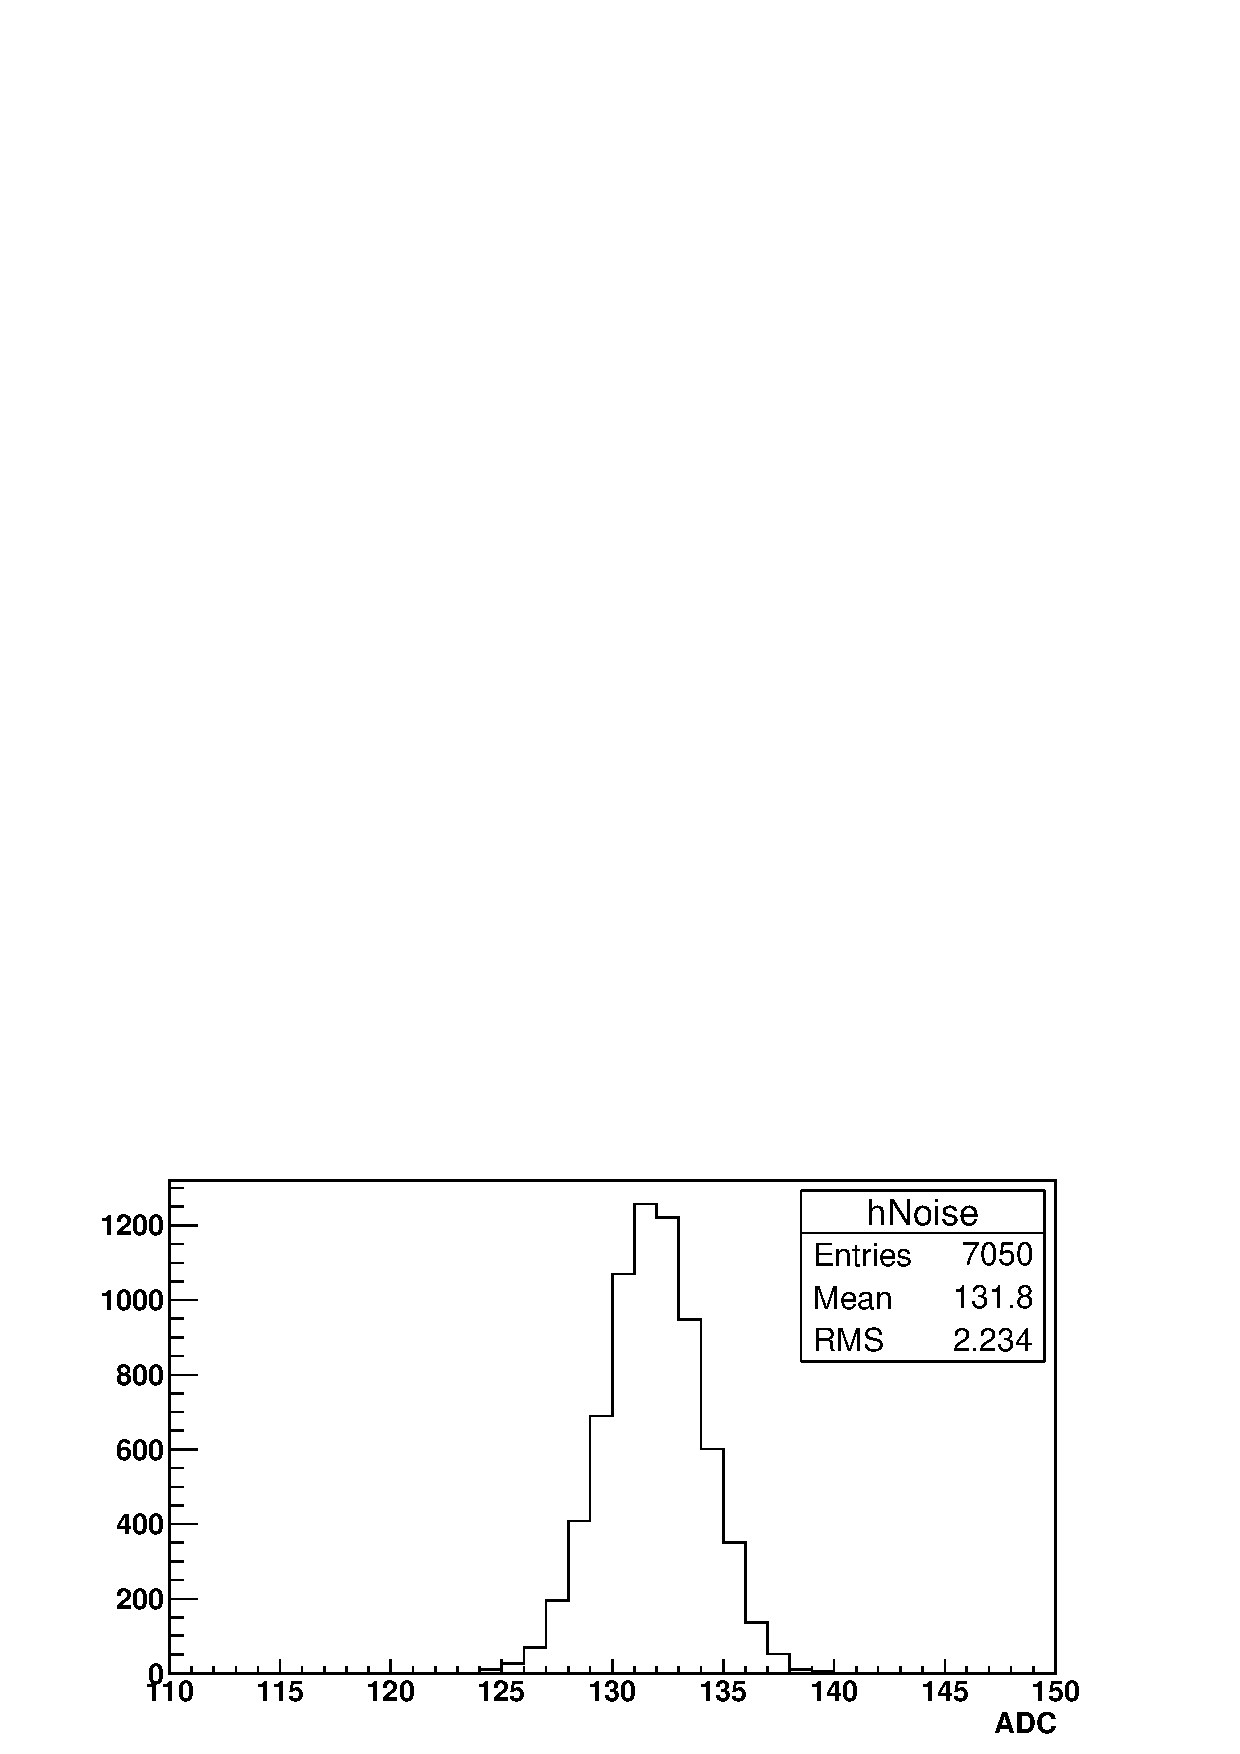
\includegraphics[width=\textwidth]{chapters/graphs/GainVarsMeas/LL_m04_2016-06-11/example_NoiseHist1.pdf}
\caption{}
\end{subfigure}
\vspace{3mm}
\begin{subfigure}[b]{0.95\textwidth}
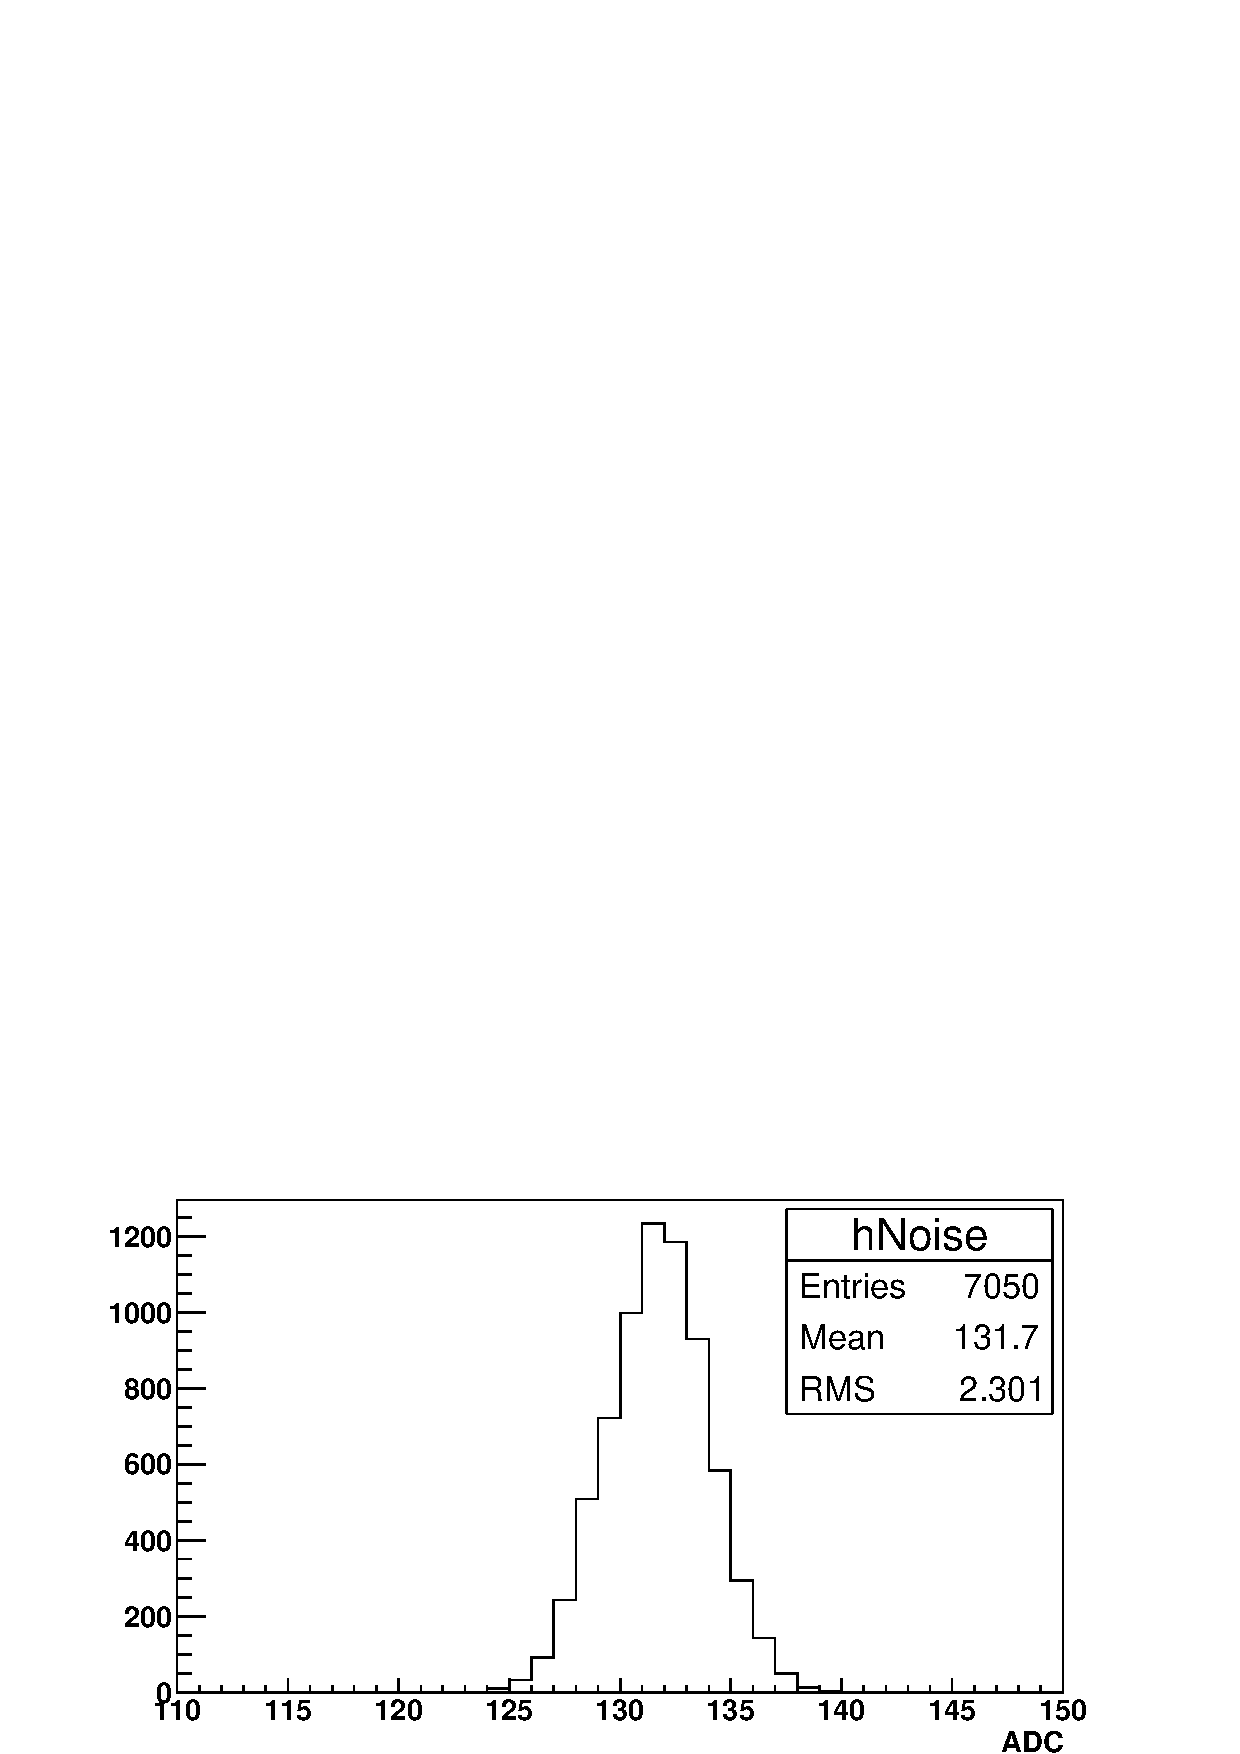
\includegraphics[width=\textwidth]{chapters/graphs/GainVarsMeas/LL_m04_2016-06-11/example_NoiseHist2.pdf}
\caption{}
\end{subfigure}
\caption{Sample of the observed electronic noise observed for a single pixel within Los Leones telescope 4.}
\end{figure}

\section{Pairs Method}

For both standard and reduced voltage settings 50 sets of pulses are recorded for the CalA analysis. The pair method

\subsection{Results}

\begin{figure} % Mean Plot
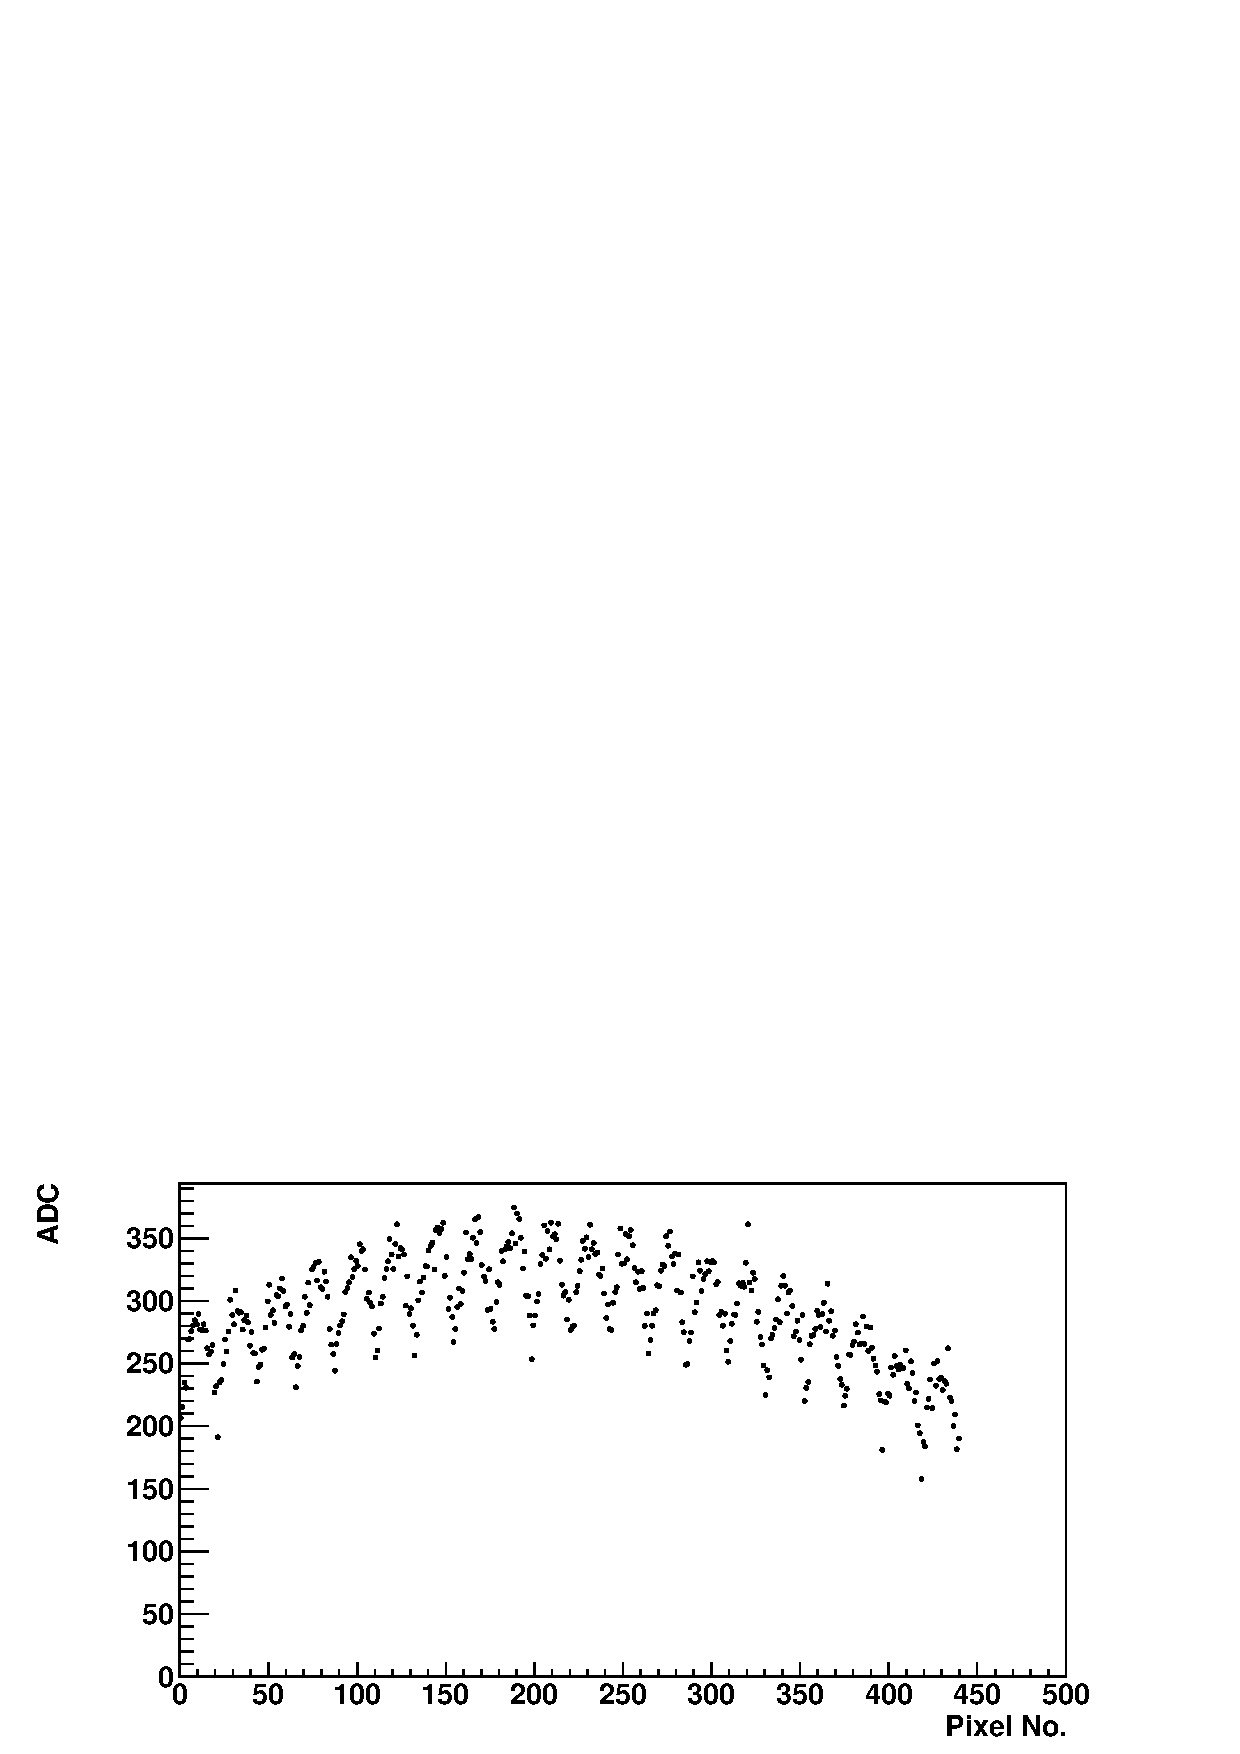
\includegraphics[width=\textwidth]{chapters/graphs/GainVarsMeas/LL_m04_2016-06-11/Set0and2/meanHist_StandHV_Pairs_set0and2.pdf}
\caption{}
\vspace{3mm}
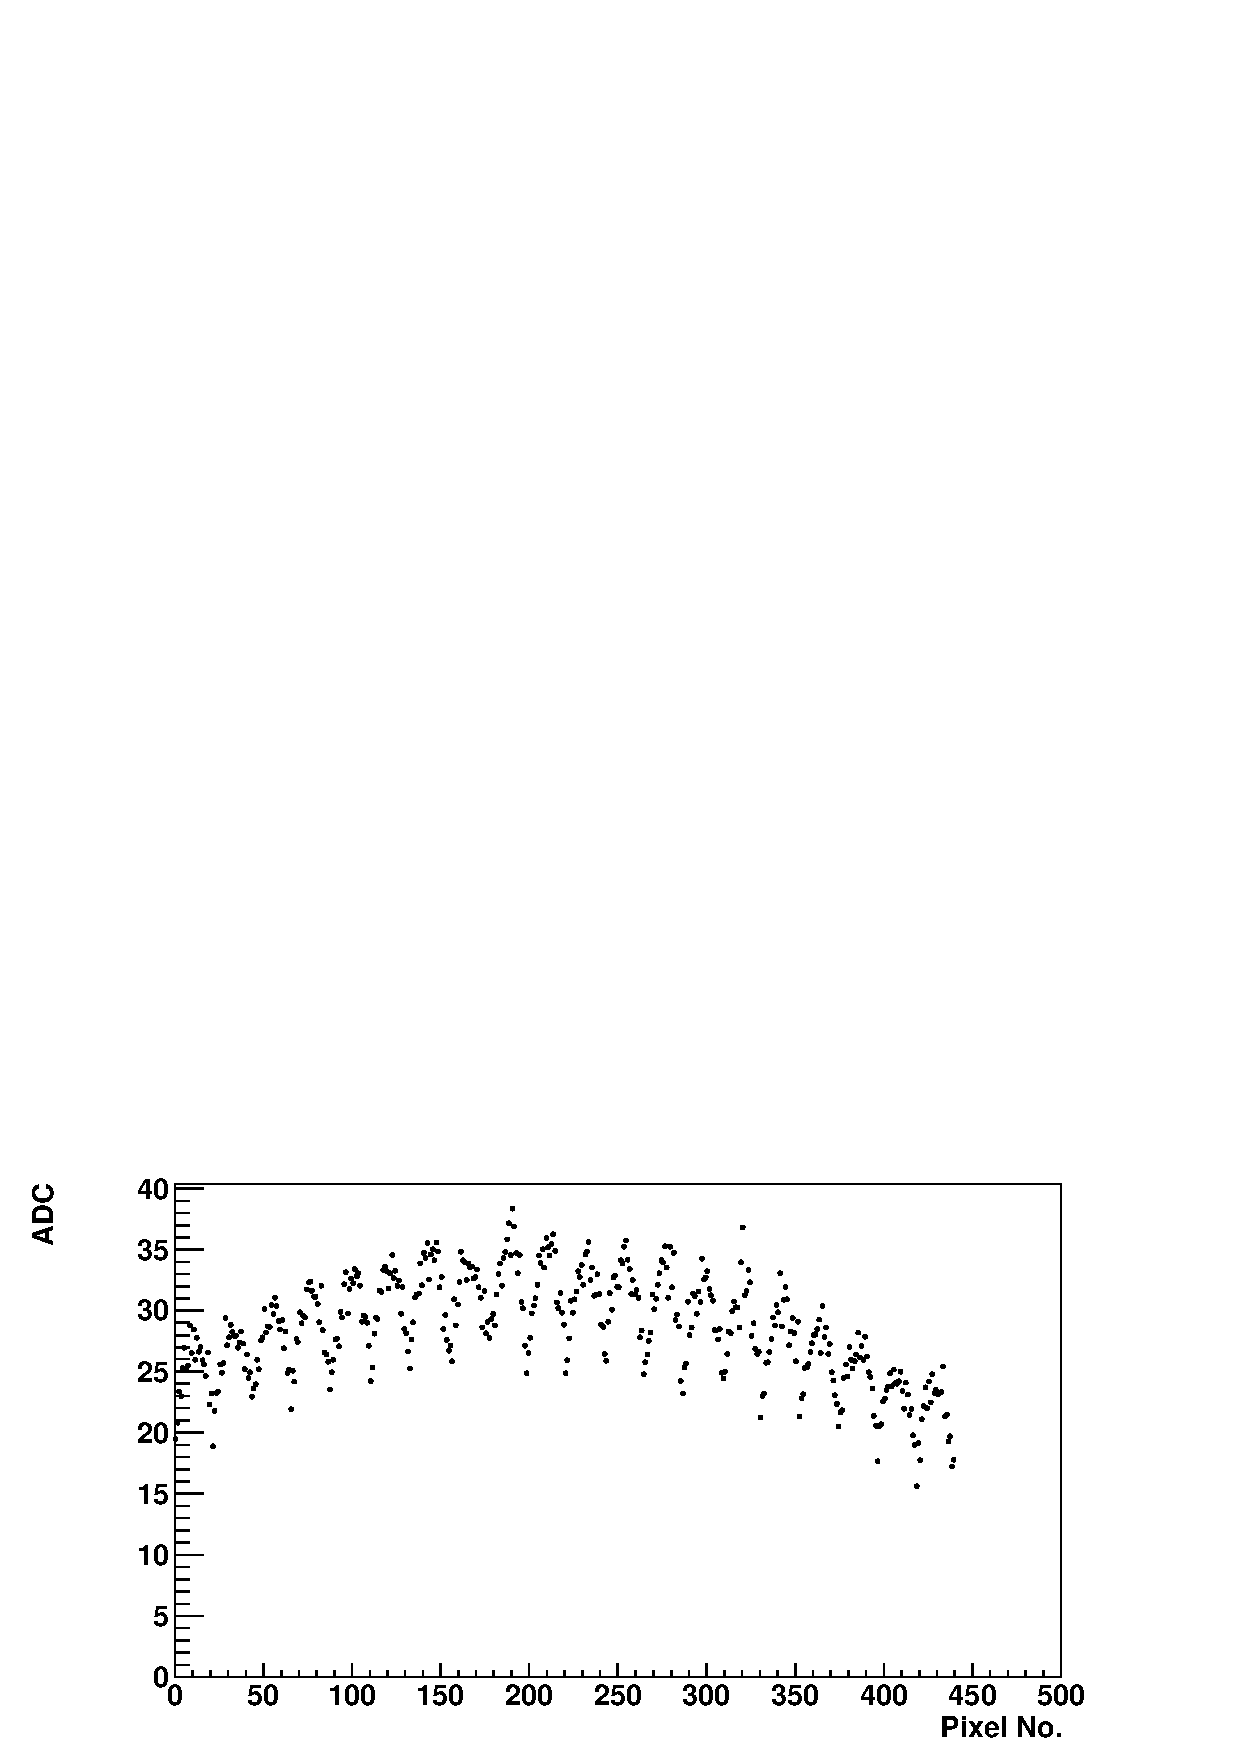
\includegraphics[width=\textwidth]{chapters/graphs/GainVarsMeas/LL_m04_2016-06-11/Set0and2/meanHist_LowHV_Pairs_set0and2.pdf}
\caption{}
\end{figure}

\begin{figure} % Variance Plot
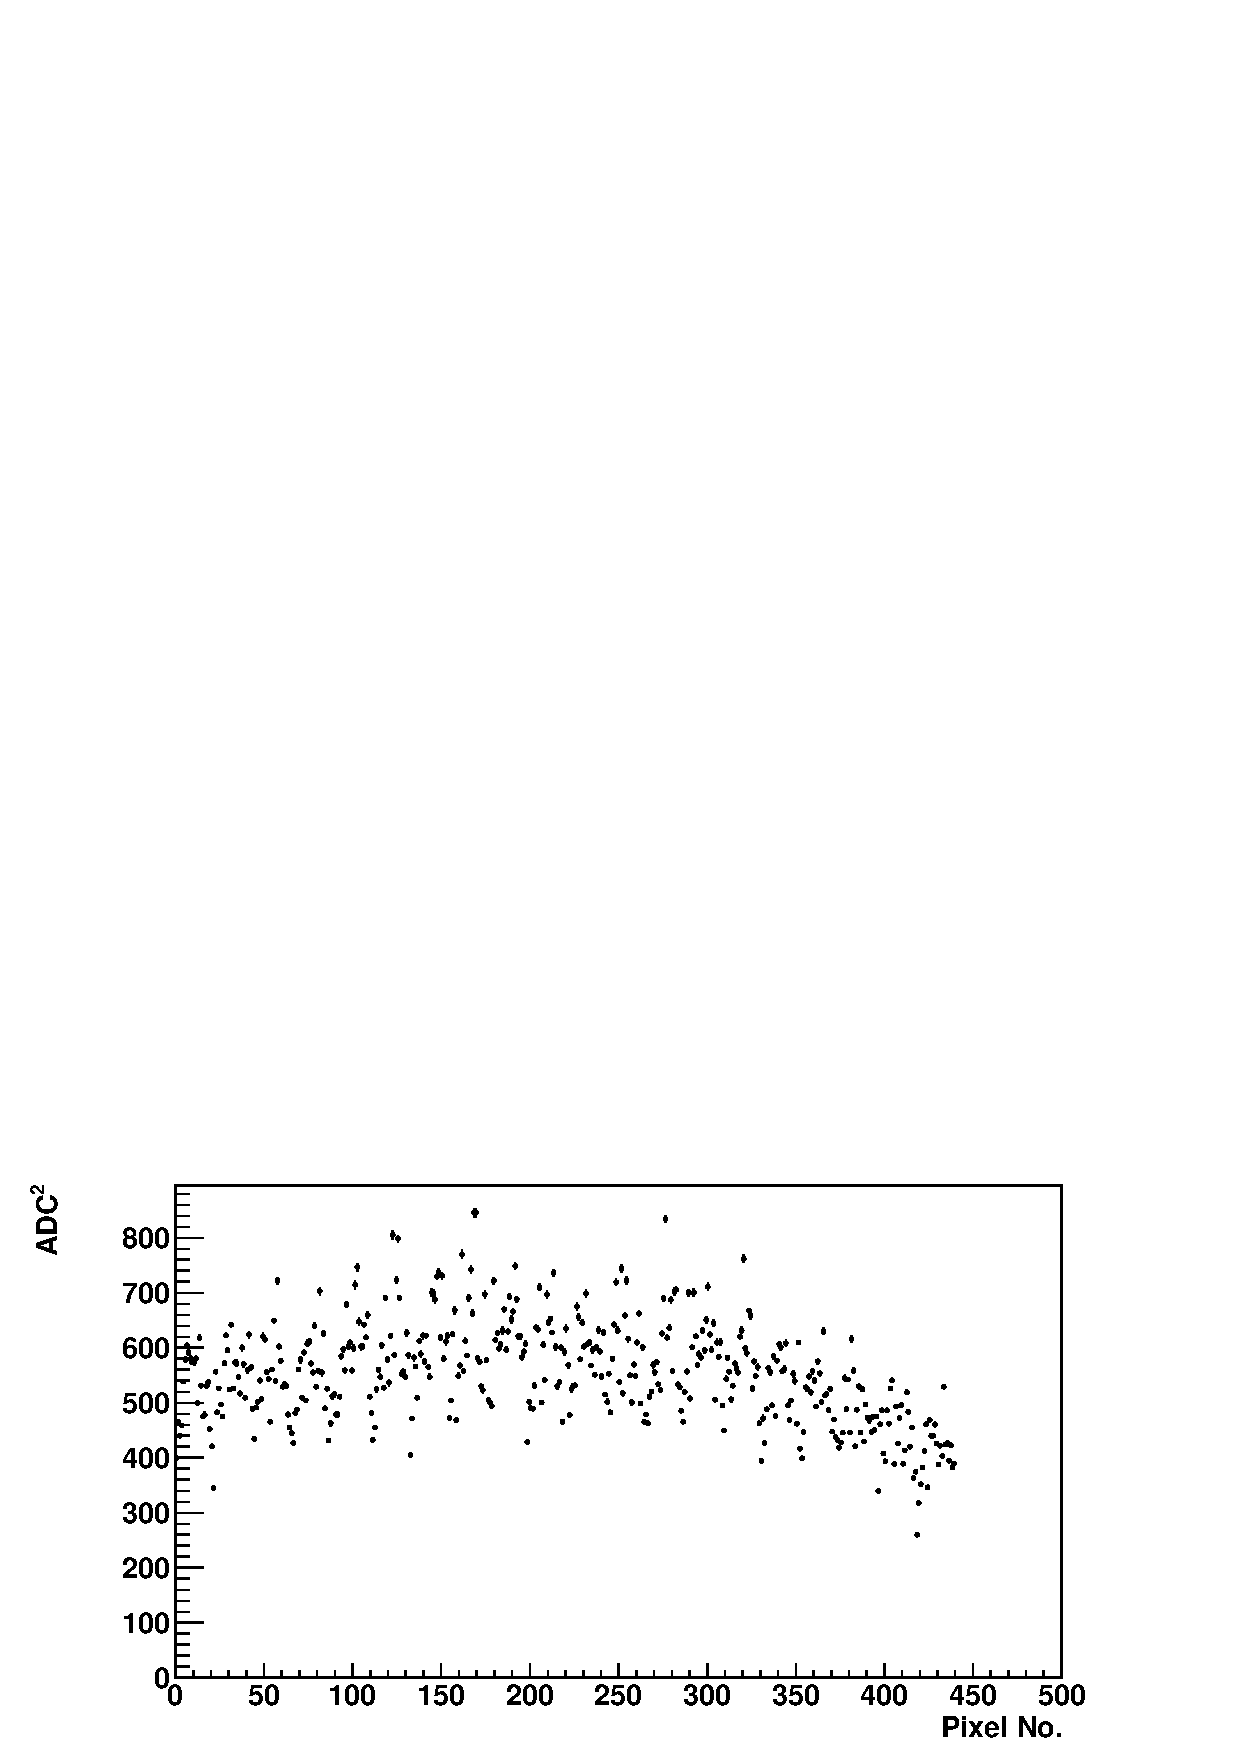
\includegraphics[width=\textwidth]{chapters/graphs/GainVarsMeas/LL_m04_2016-06-11/Set0and2/varianceHist_StandHV_Pairs_set0and2.pdf}
\caption{}
\vspace{3mm}
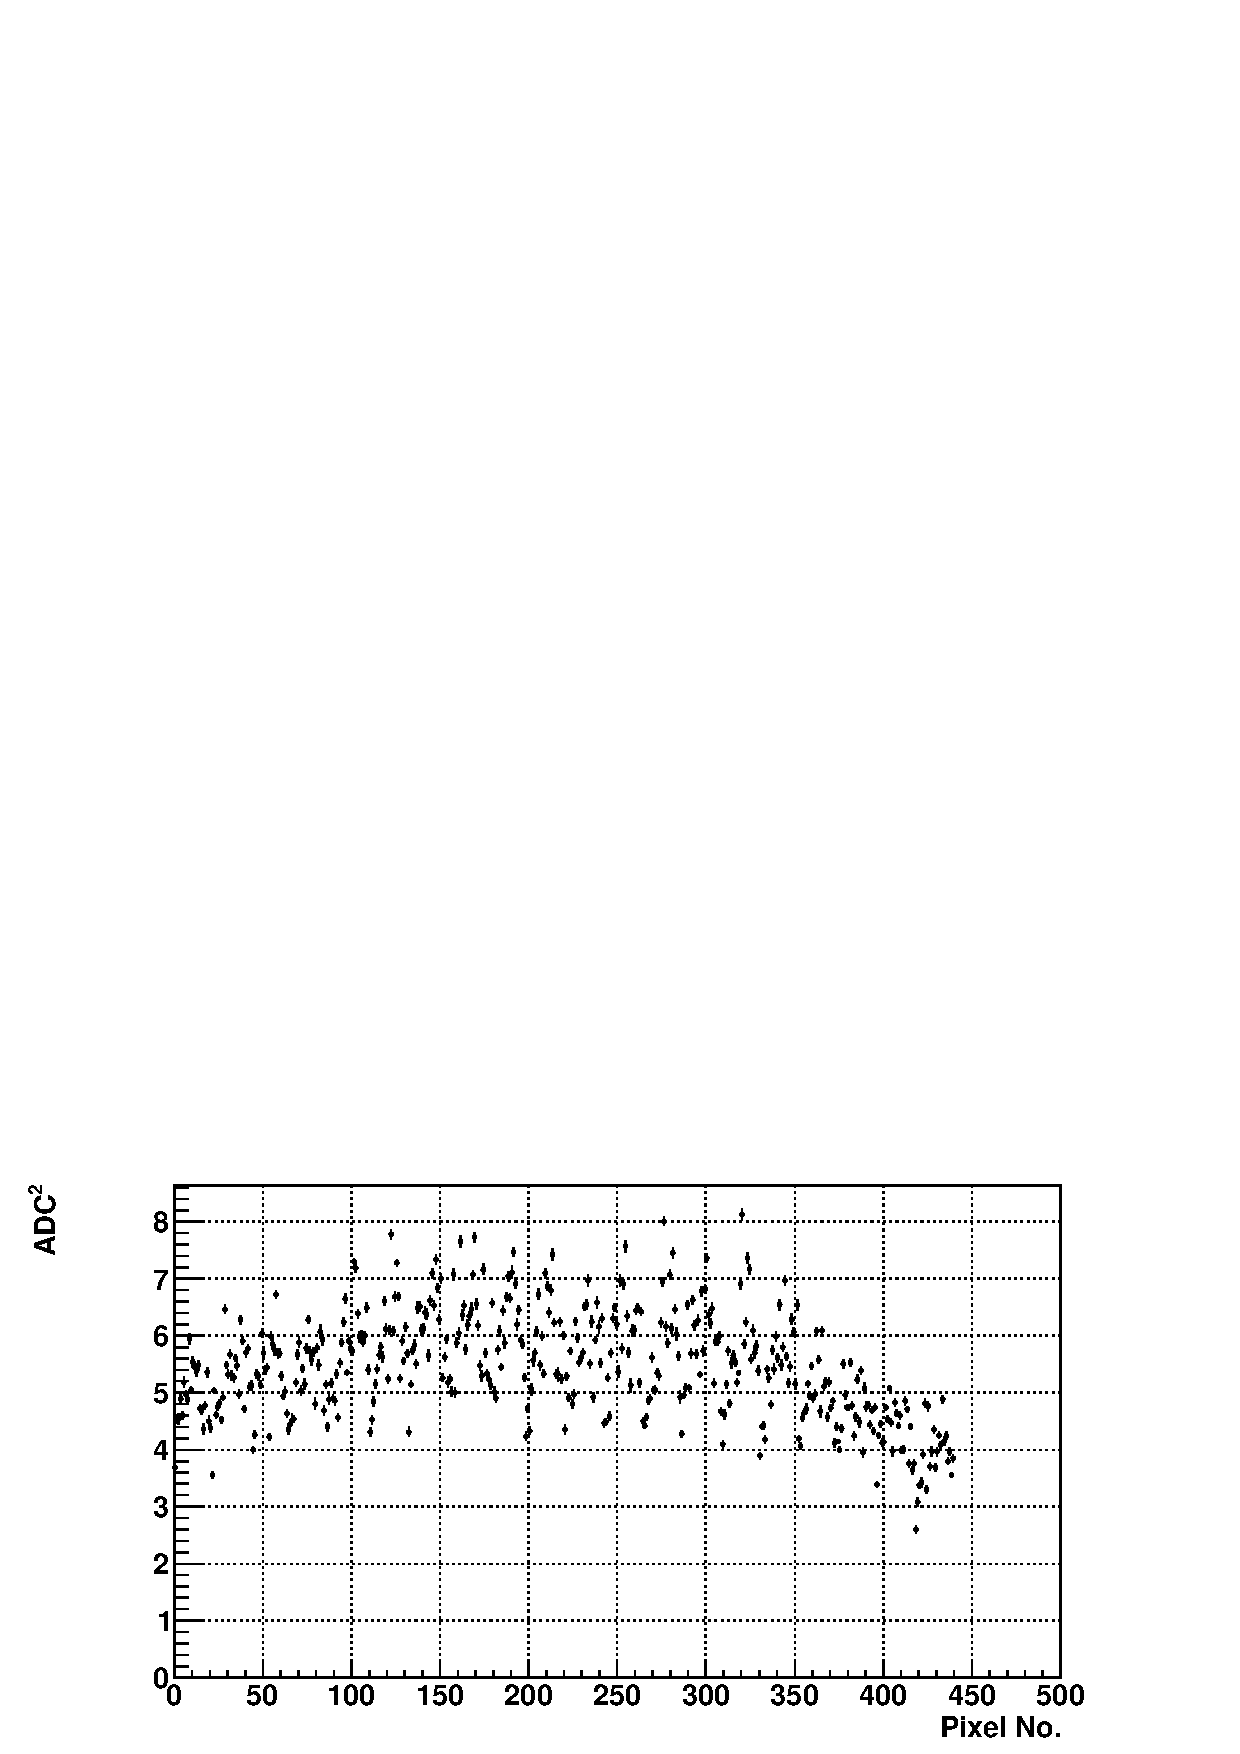
\includegraphics[width=\textwidth]{chapters/graphs/GainVarsMeas/LL_m04_2016-06-11/Set0and2/varianceHist_LowHV_Pairs_set0and2.pdf}
\caption{}
\end{figure}

\begin{figure} % Gain Variance Plot
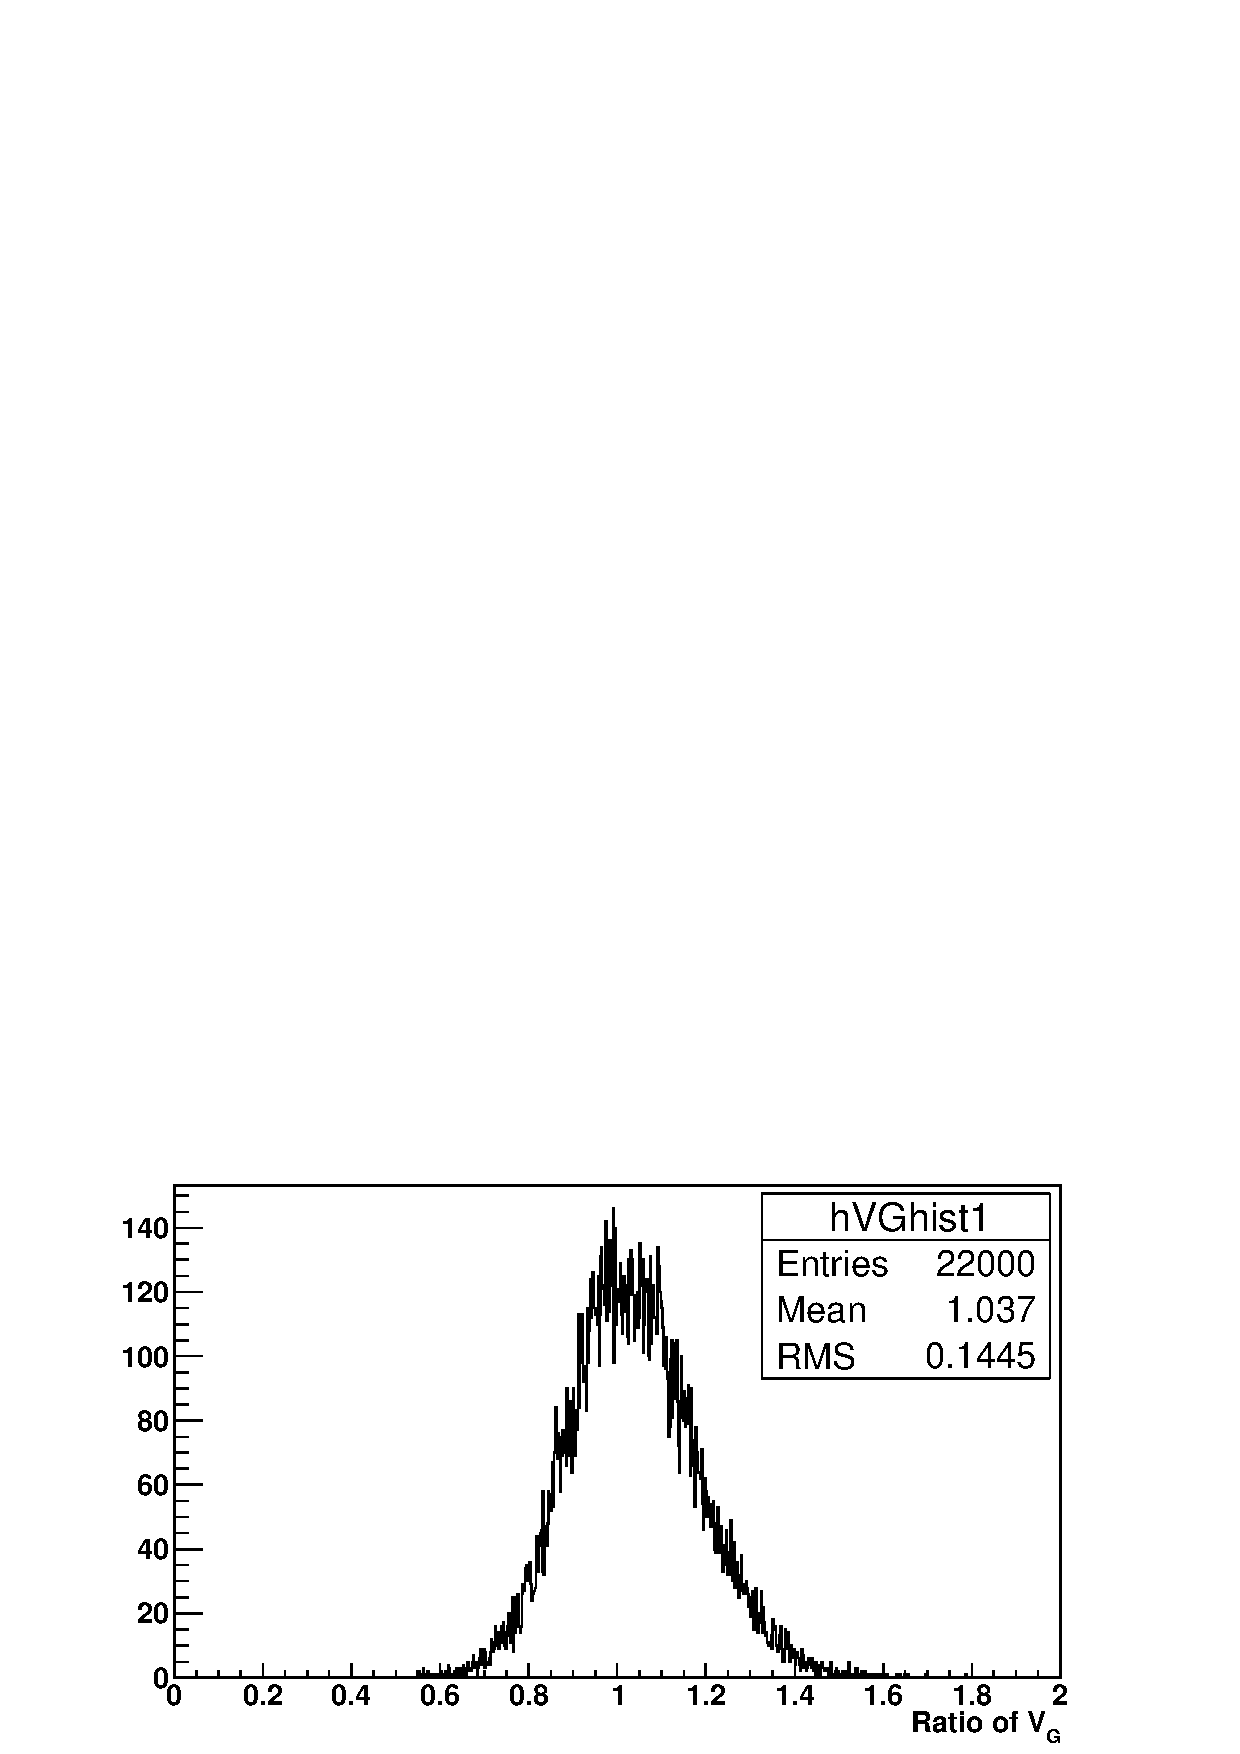
\includegraphics[width=\textwidth]{chapters/graphs/GainVarsMeas/LL_m04_2016-06-11/Set0and2/GainVairanceHist_Pairs.pdf}
\caption{}
\vspace{3mm}
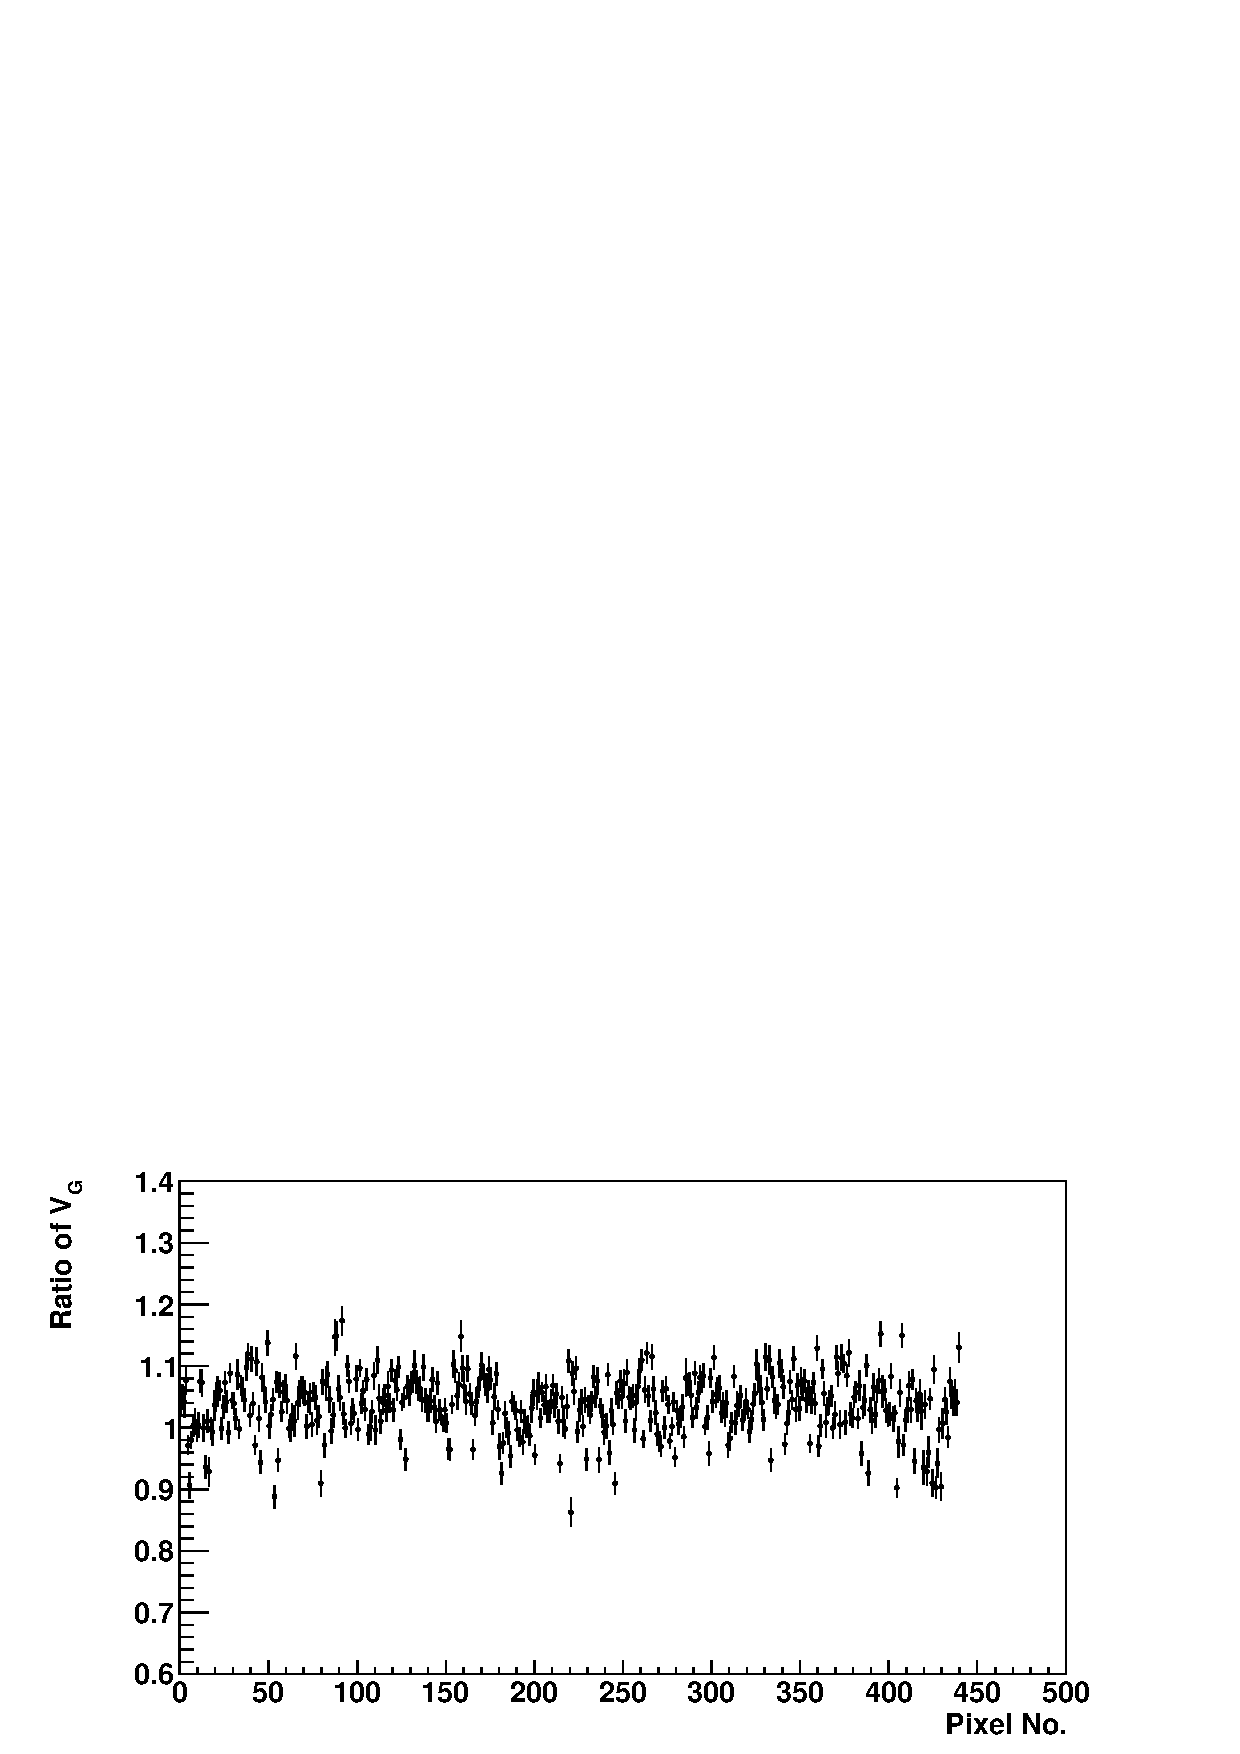
\includegraphics[width=\textwidth]{chapters/graphs/GainVarsMeas/LL_m04_2016-06-11/Set0and2/GainVars_Vs_Pixel_GainVariance_Pairs_Set0and2.pdf}
\caption{}
\end{figure}

\section{Result of Averaging Sets of Traces Method}

\begin{figure} % Mean Plot
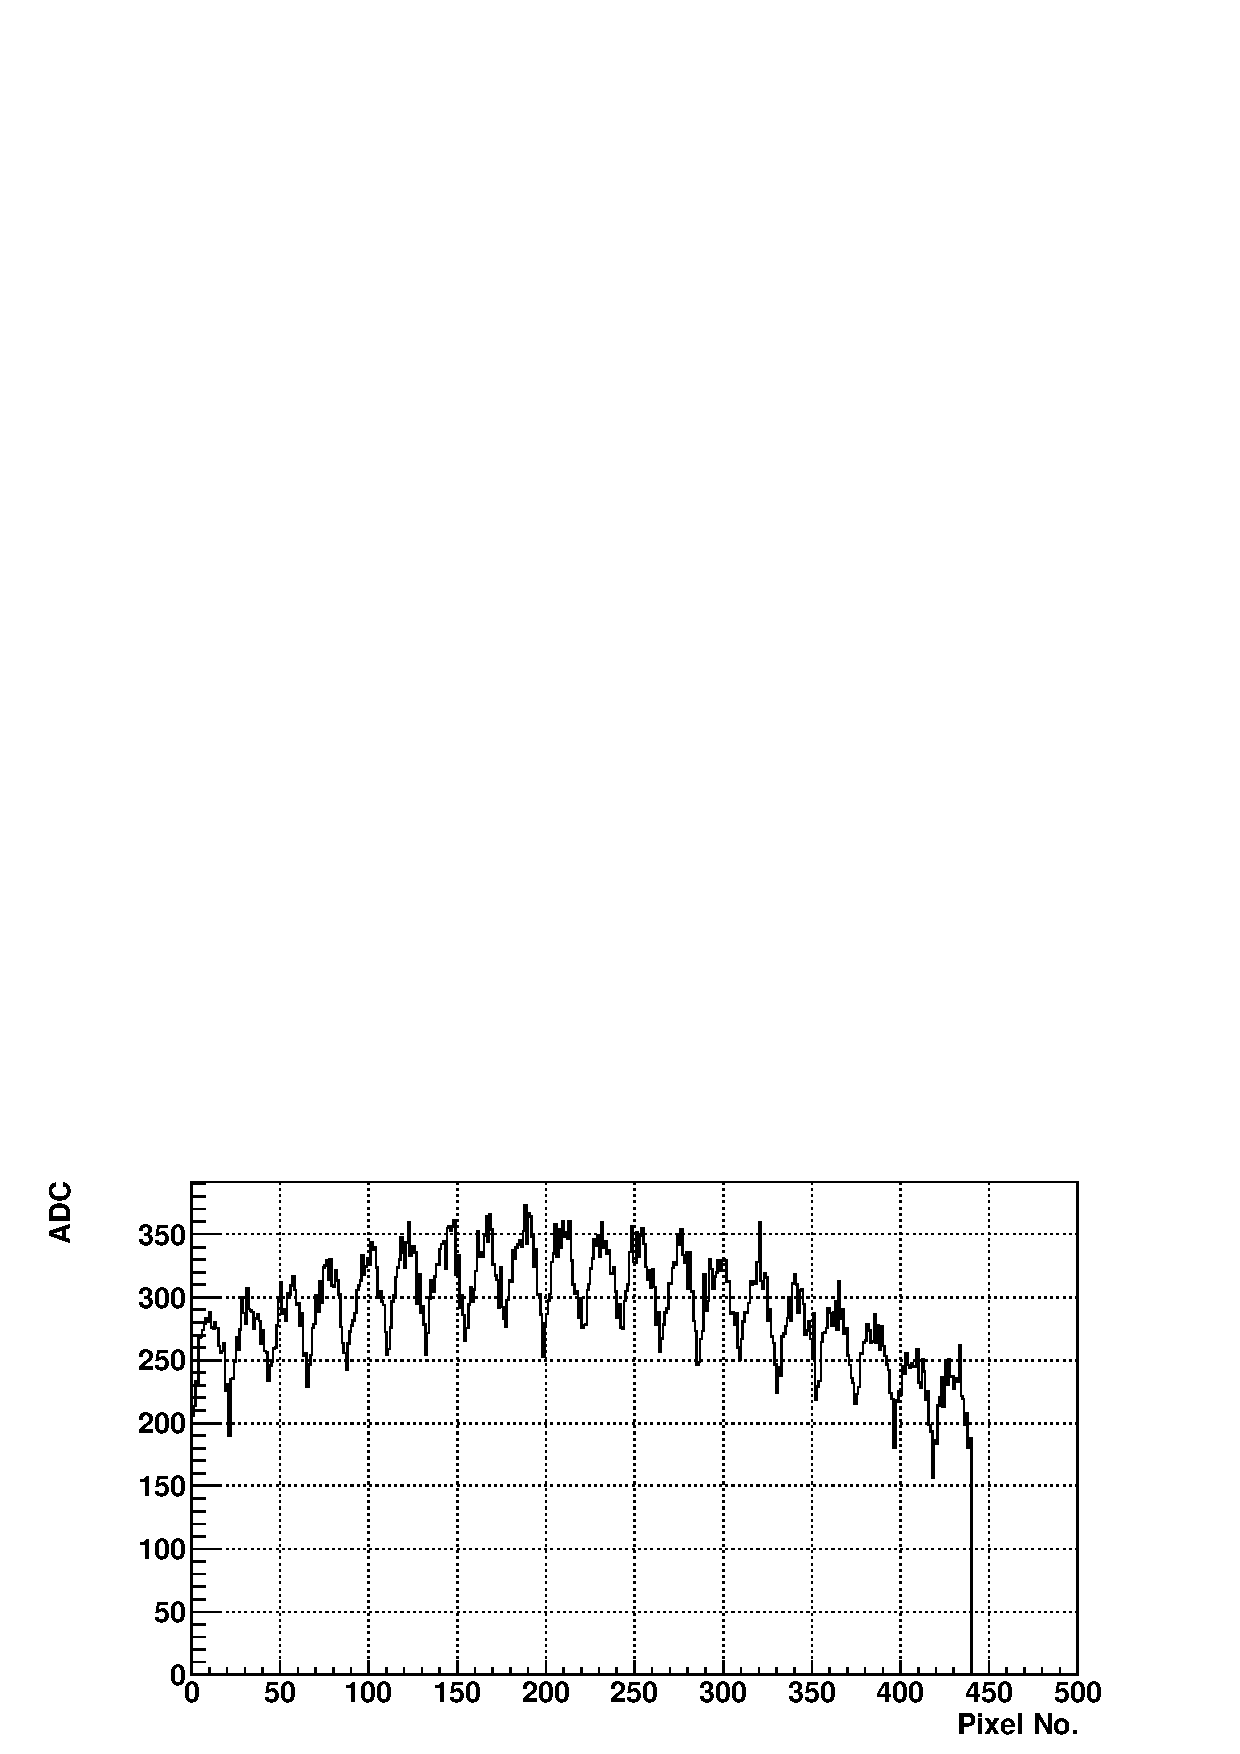
\includegraphics[width=\textwidth]{chapters/graphs/GainVarsMeas/LL_m04_2016-06-11/Set0and2/meanHist_StandHV_Average_set0and2.pdf}
\caption{}
\vspace{3mm}
\includegraphics[width=\textwidth]{chapters/graphs/GainVarsMeas/LL_m04_2016-06-11/Set0and2/meanHist_LowHV_Average_set0and2.pdf}
\caption{}
\end{figure}

\begin{figure} % Variance Plot
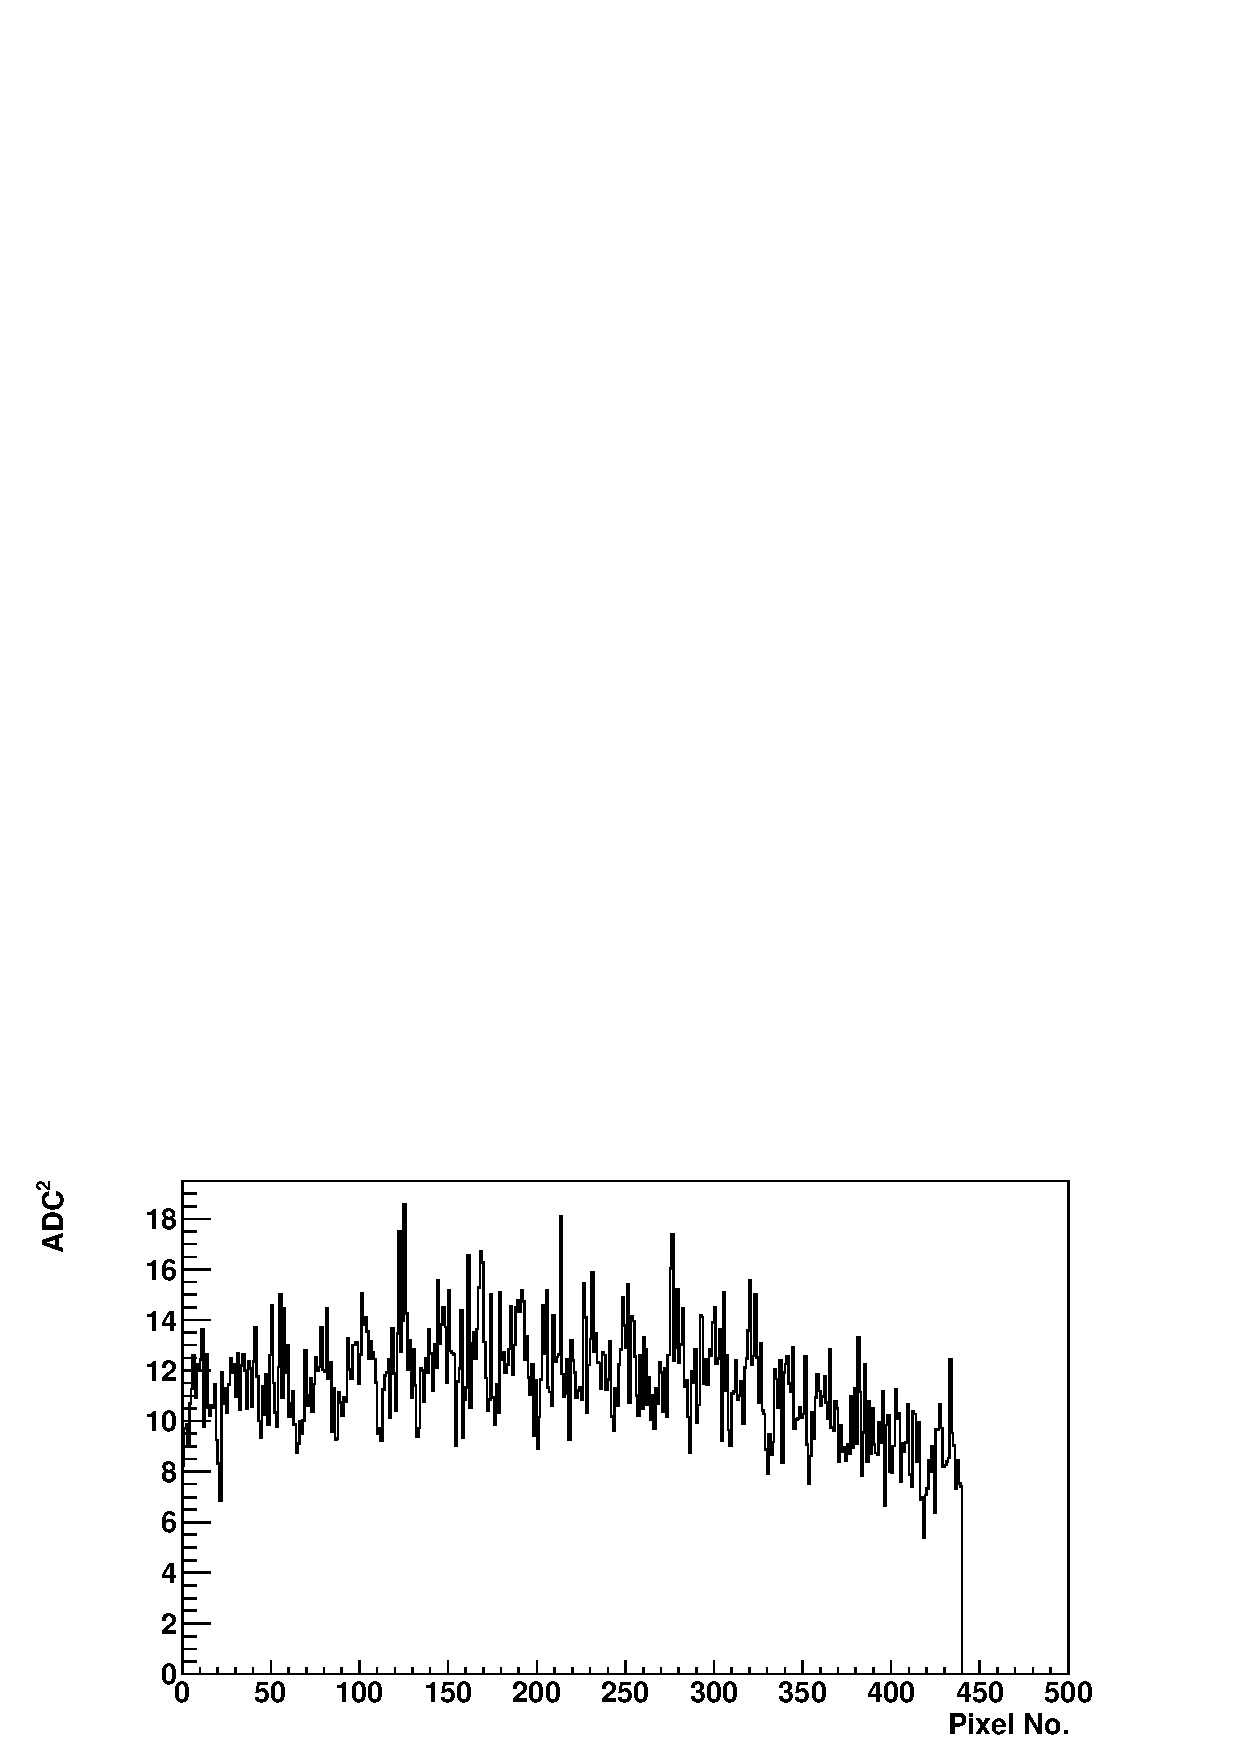
\includegraphics[width=\textwidth]{chapters/graphs/GainVarsMeas/LL_m04_2016-06-11/Set0and2/varianceHist_StandHV_Average_set0and2.pdf}
\caption{}
\vspace{3mm}
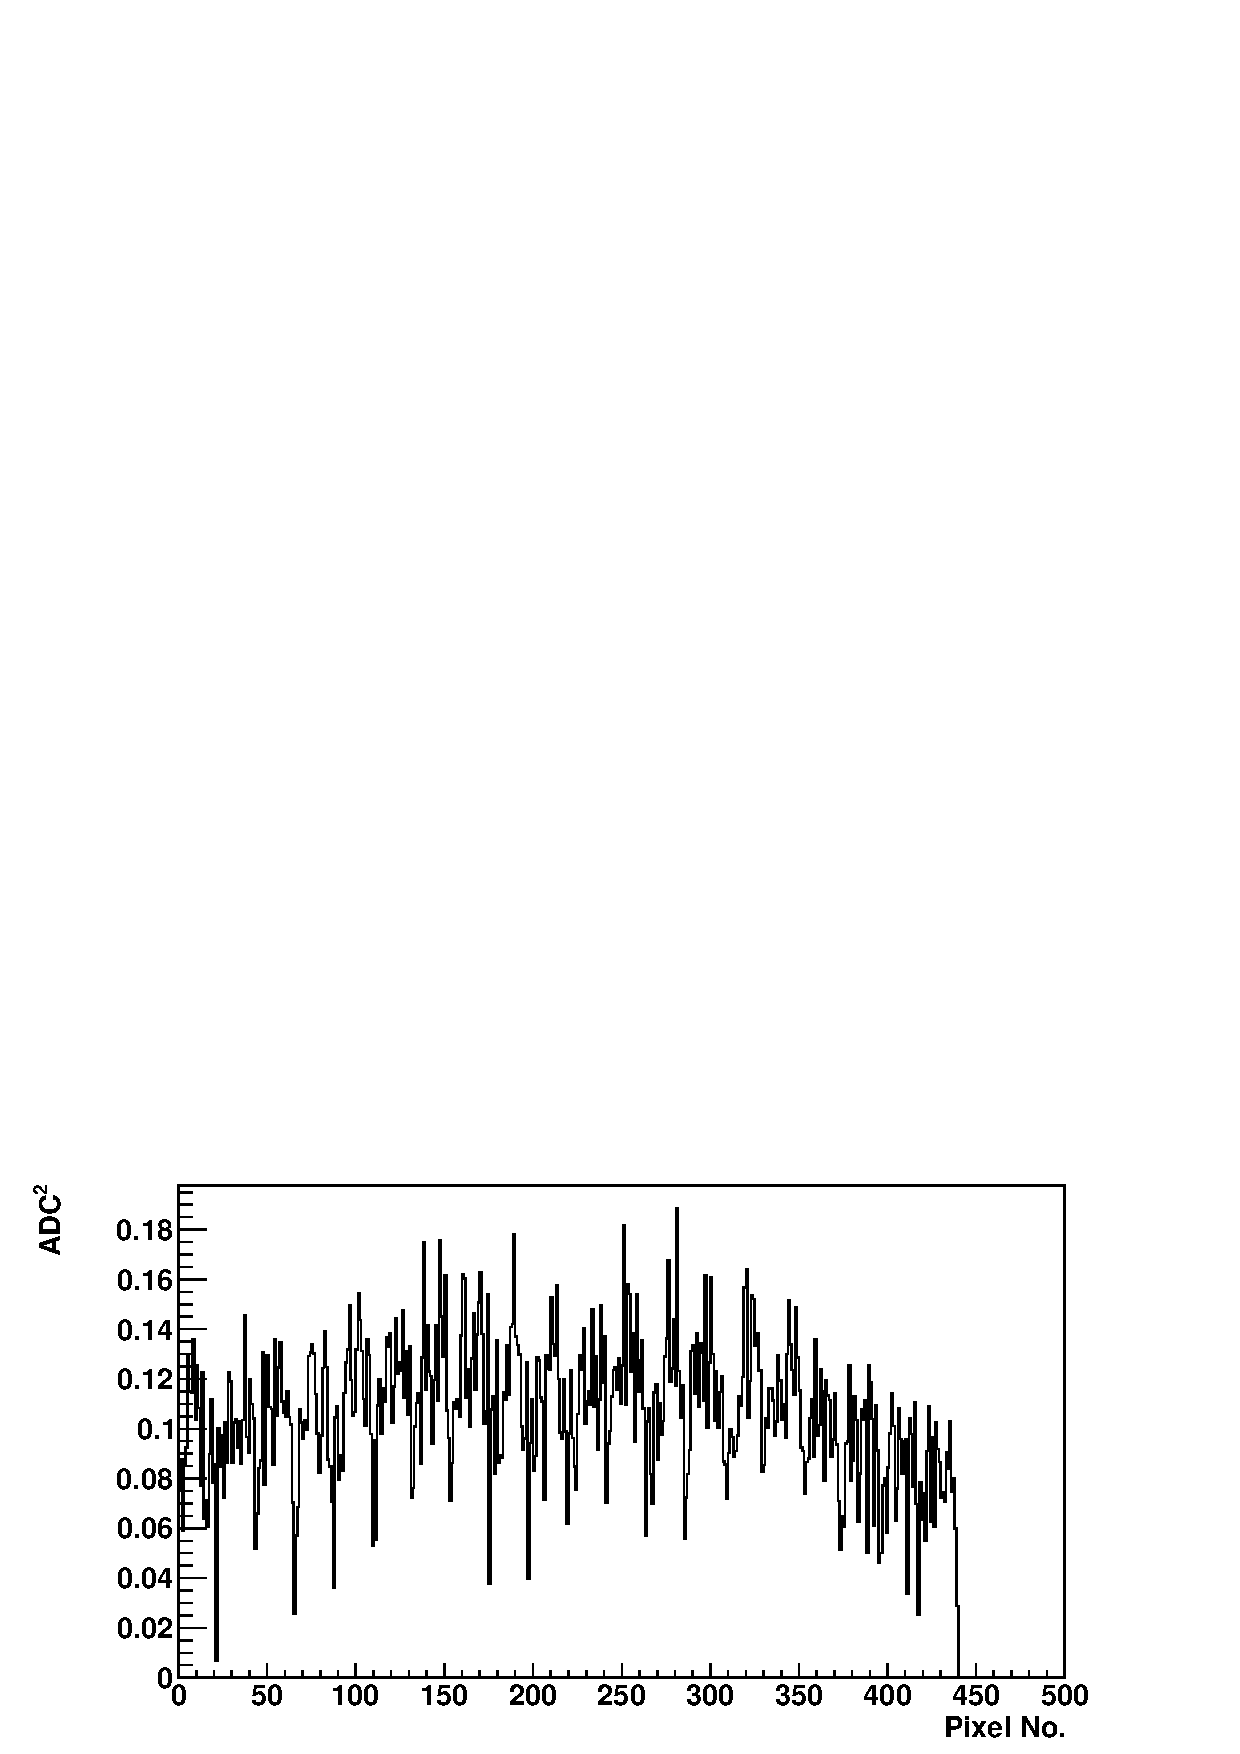
\includegraphics[width=\textwidth]{chapters/graphs/GainVarsMeas/LL_m04_2016-06-11/Set0and2/varianceHist_LowHV_Average_set0and2.pdf}
\caption{}
\end{figure}

\begin{figure} % Gain Variance Plot
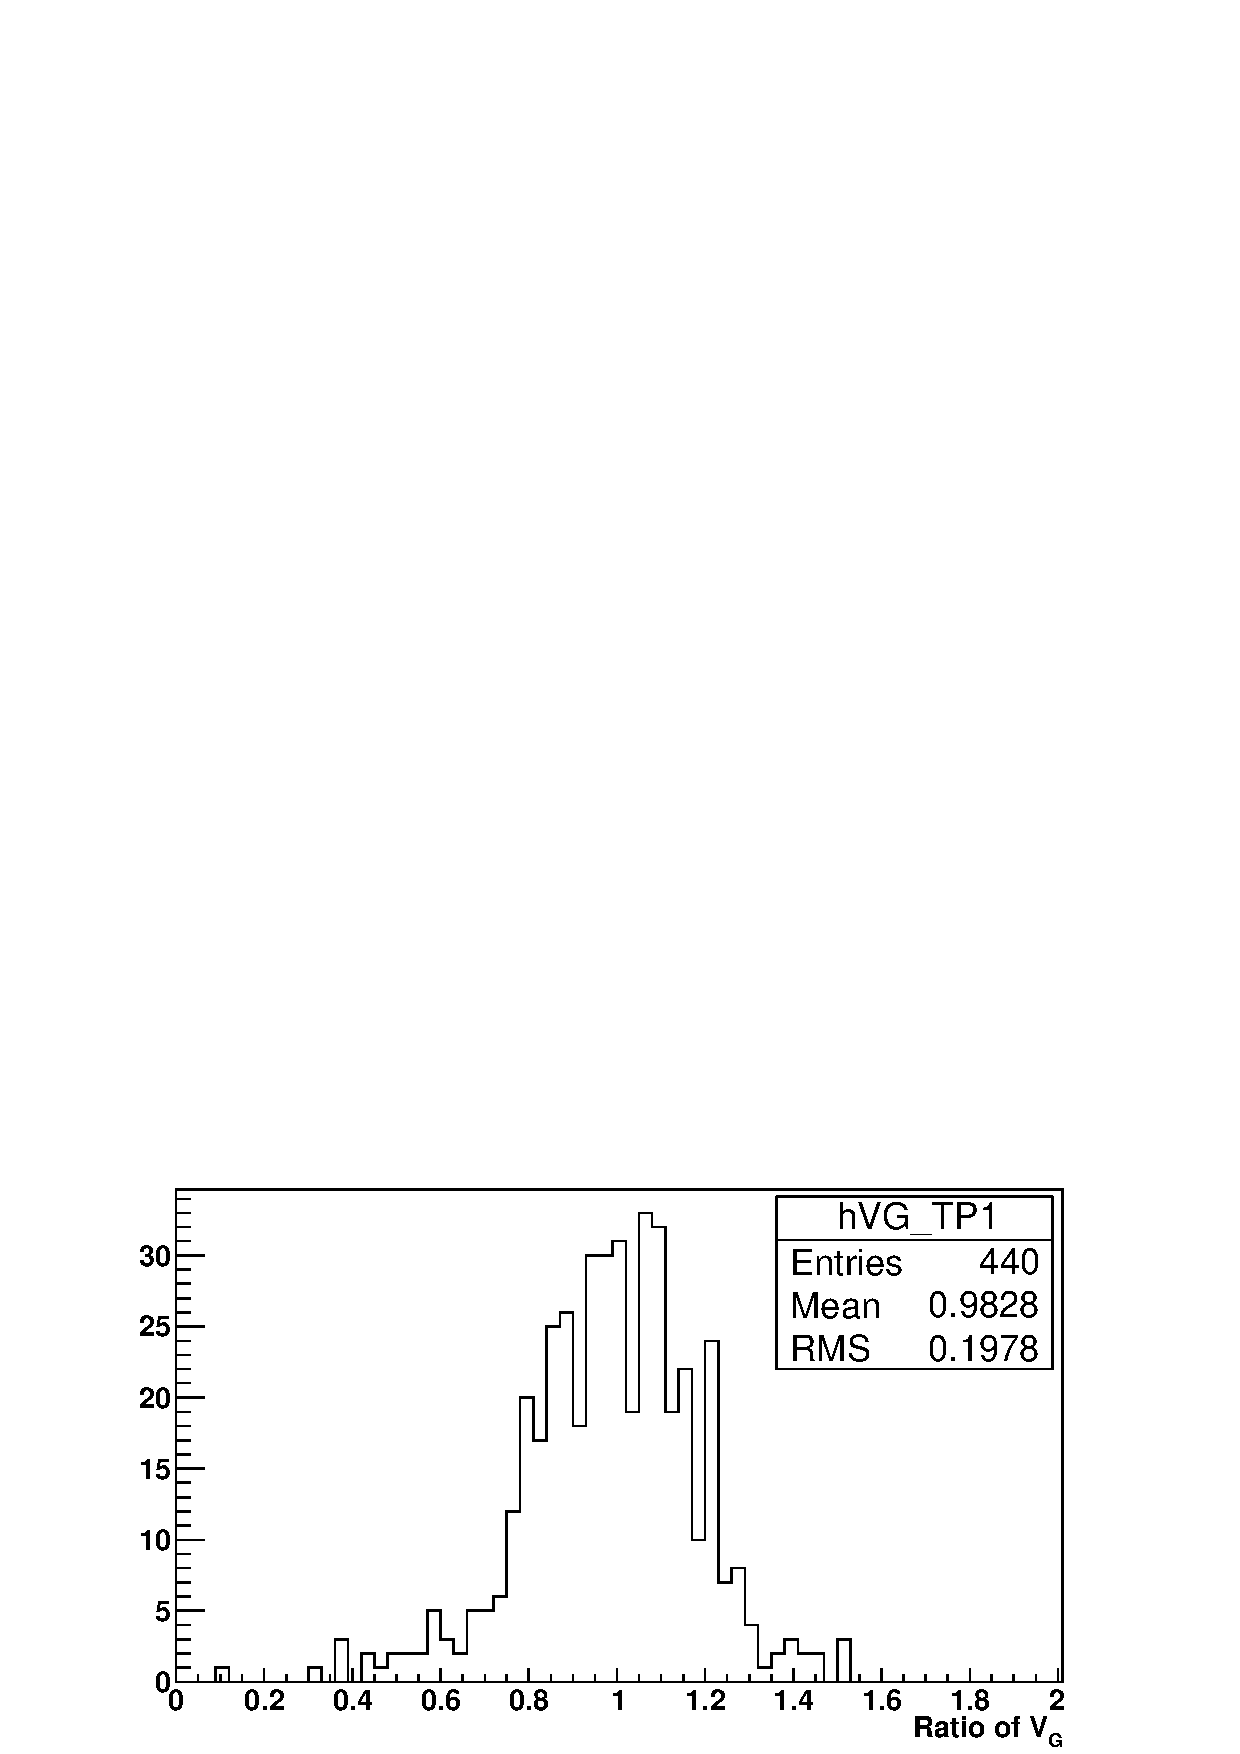
\includegraphics[width=\textwidth]{chapters/graphs/GainVarsMeas/LL_m04_2016-06-11/Set0and2/GainVairanceHist_Average_Method1.pdf}
\caption{}
\vspace{3mm}
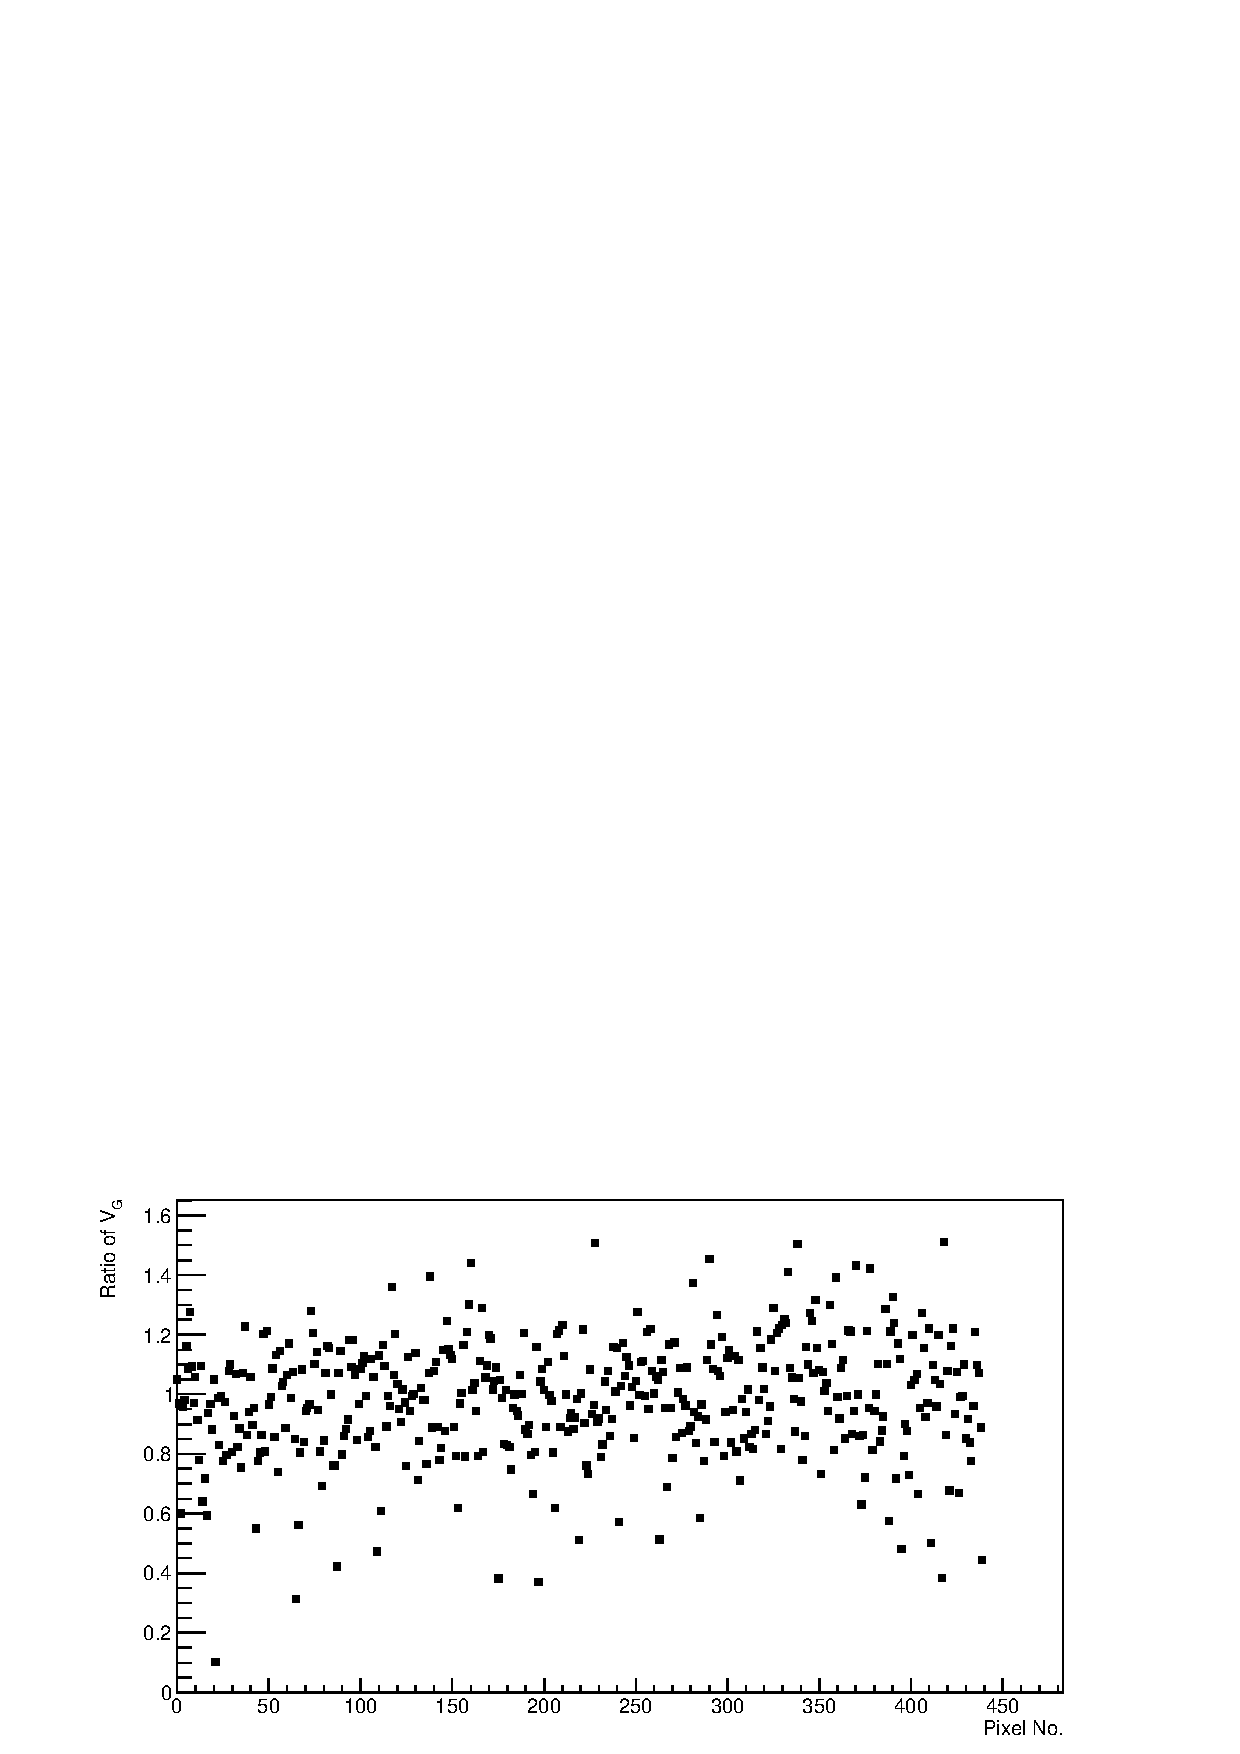
\includegraphics[width=\textwidth]{chapters/graphs/GainVarsMeas/LL_m04_2016-06-11/Set0and2/GainVars_Vs_Pixel_GainVariance_Average_Method1_Set0and2.pdf}
\caption{}
\end{figure}

\section{Result of Averaging Sets of Traces Method with Least Trimmed Squares}

\begin{figure}% Signal Chi2
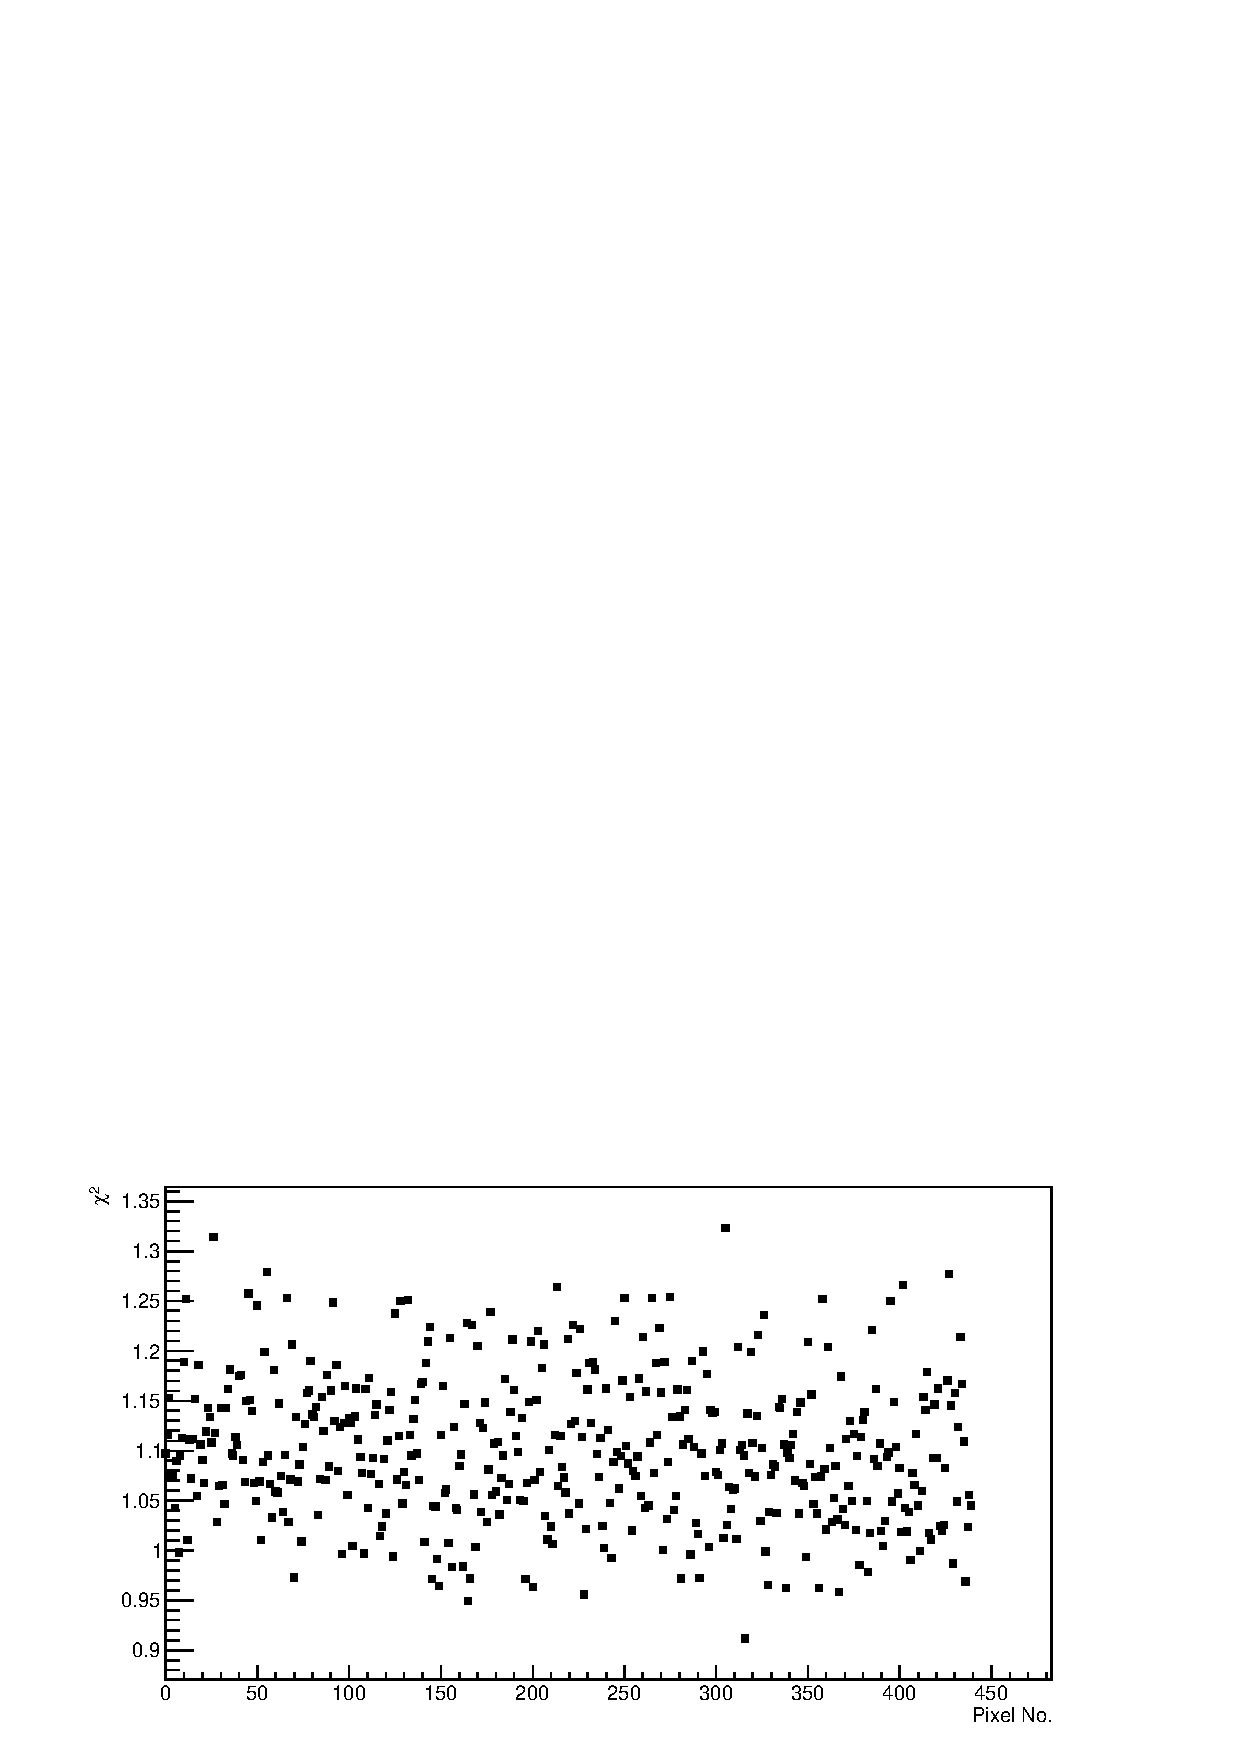
\includegraphics[width=\textwidth]{chapters/graphs/GainVarsMeas/LL_m04_2016-06-11/Set0and2/Chi2_AverageMethod_Signal_StandHV.pdf}
\caption{}
\vspace{3mm}
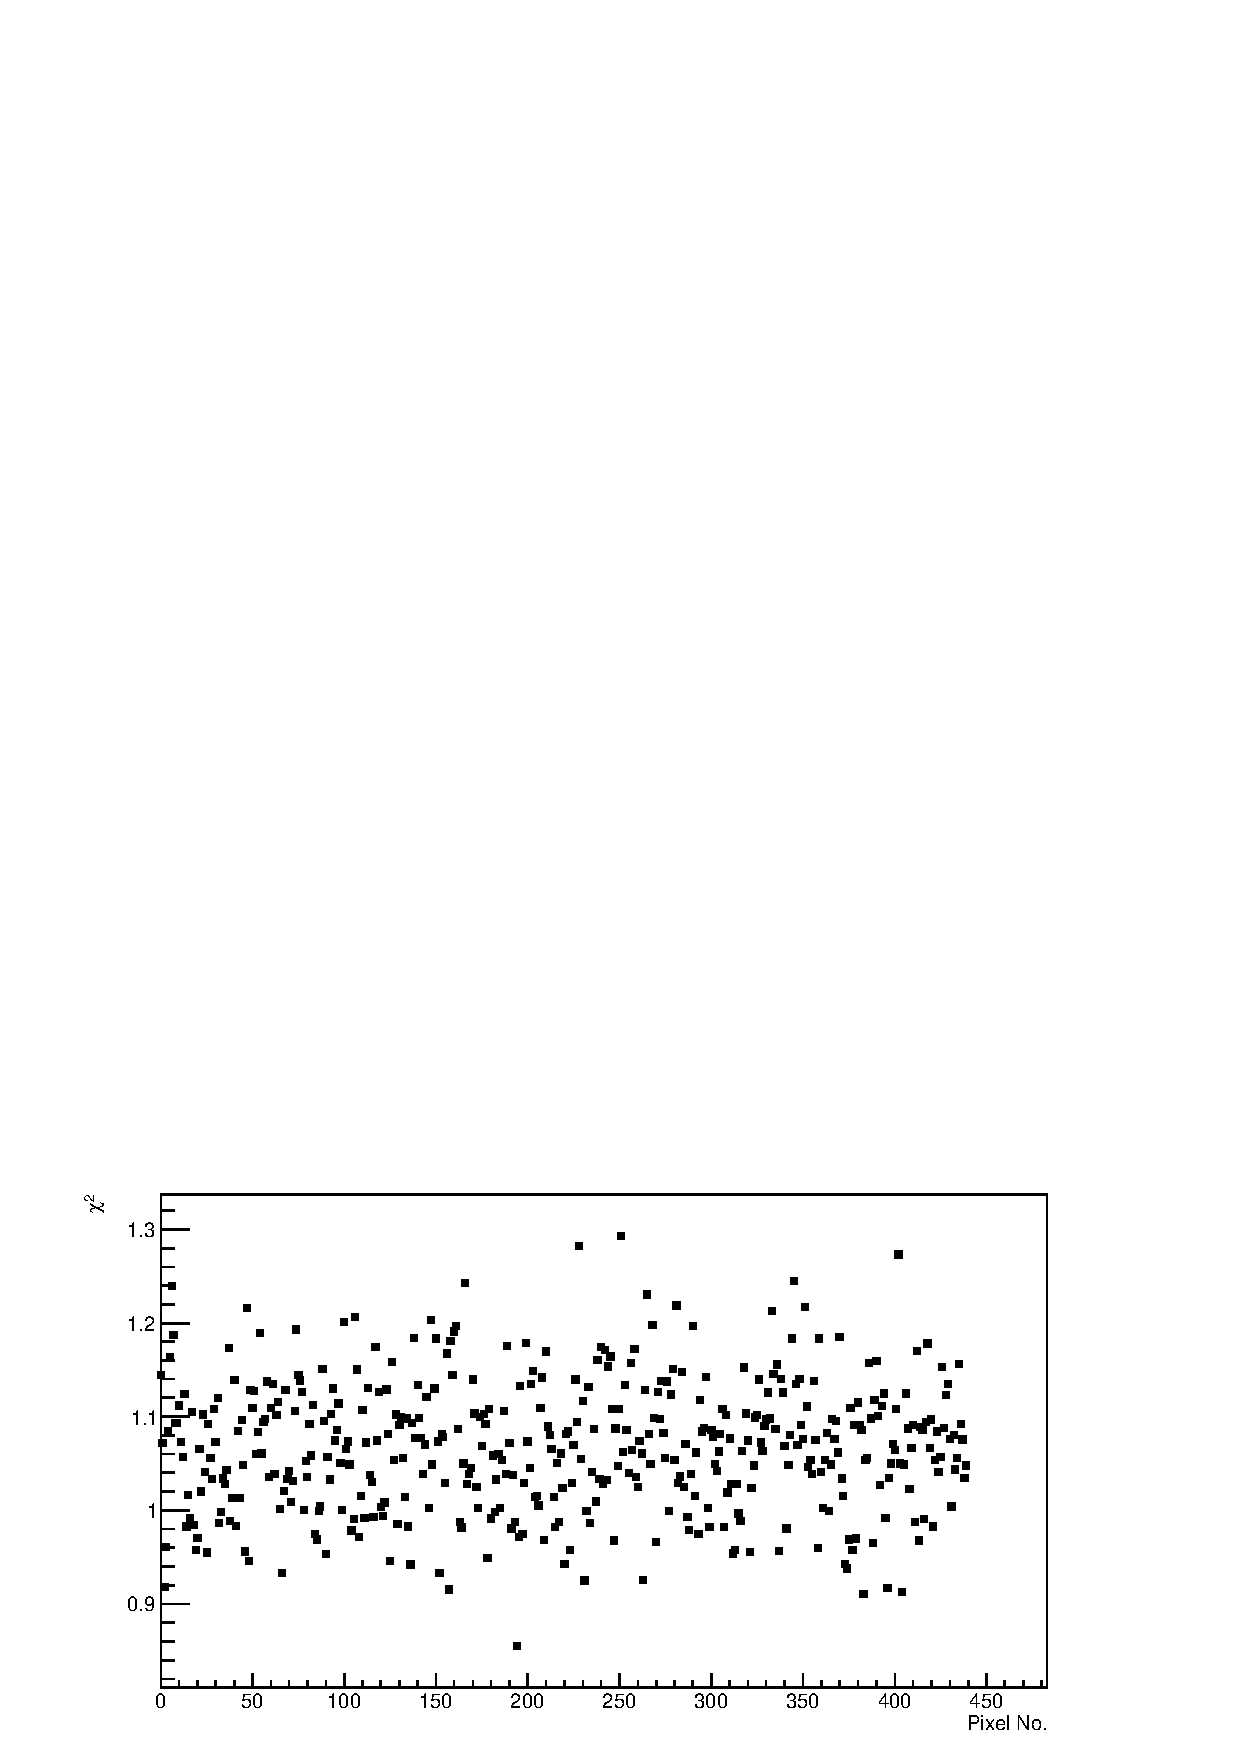
\includegraphics[width=\textwidth]{chapters/graphs/GainVarsMeas/LL_m04_2016-06-11/Set0and2/Chi2_AverageMethod_Signal_LowHV.pdf}
\caption{}
\end{figure}

\begin{figure}% Noise Chi2
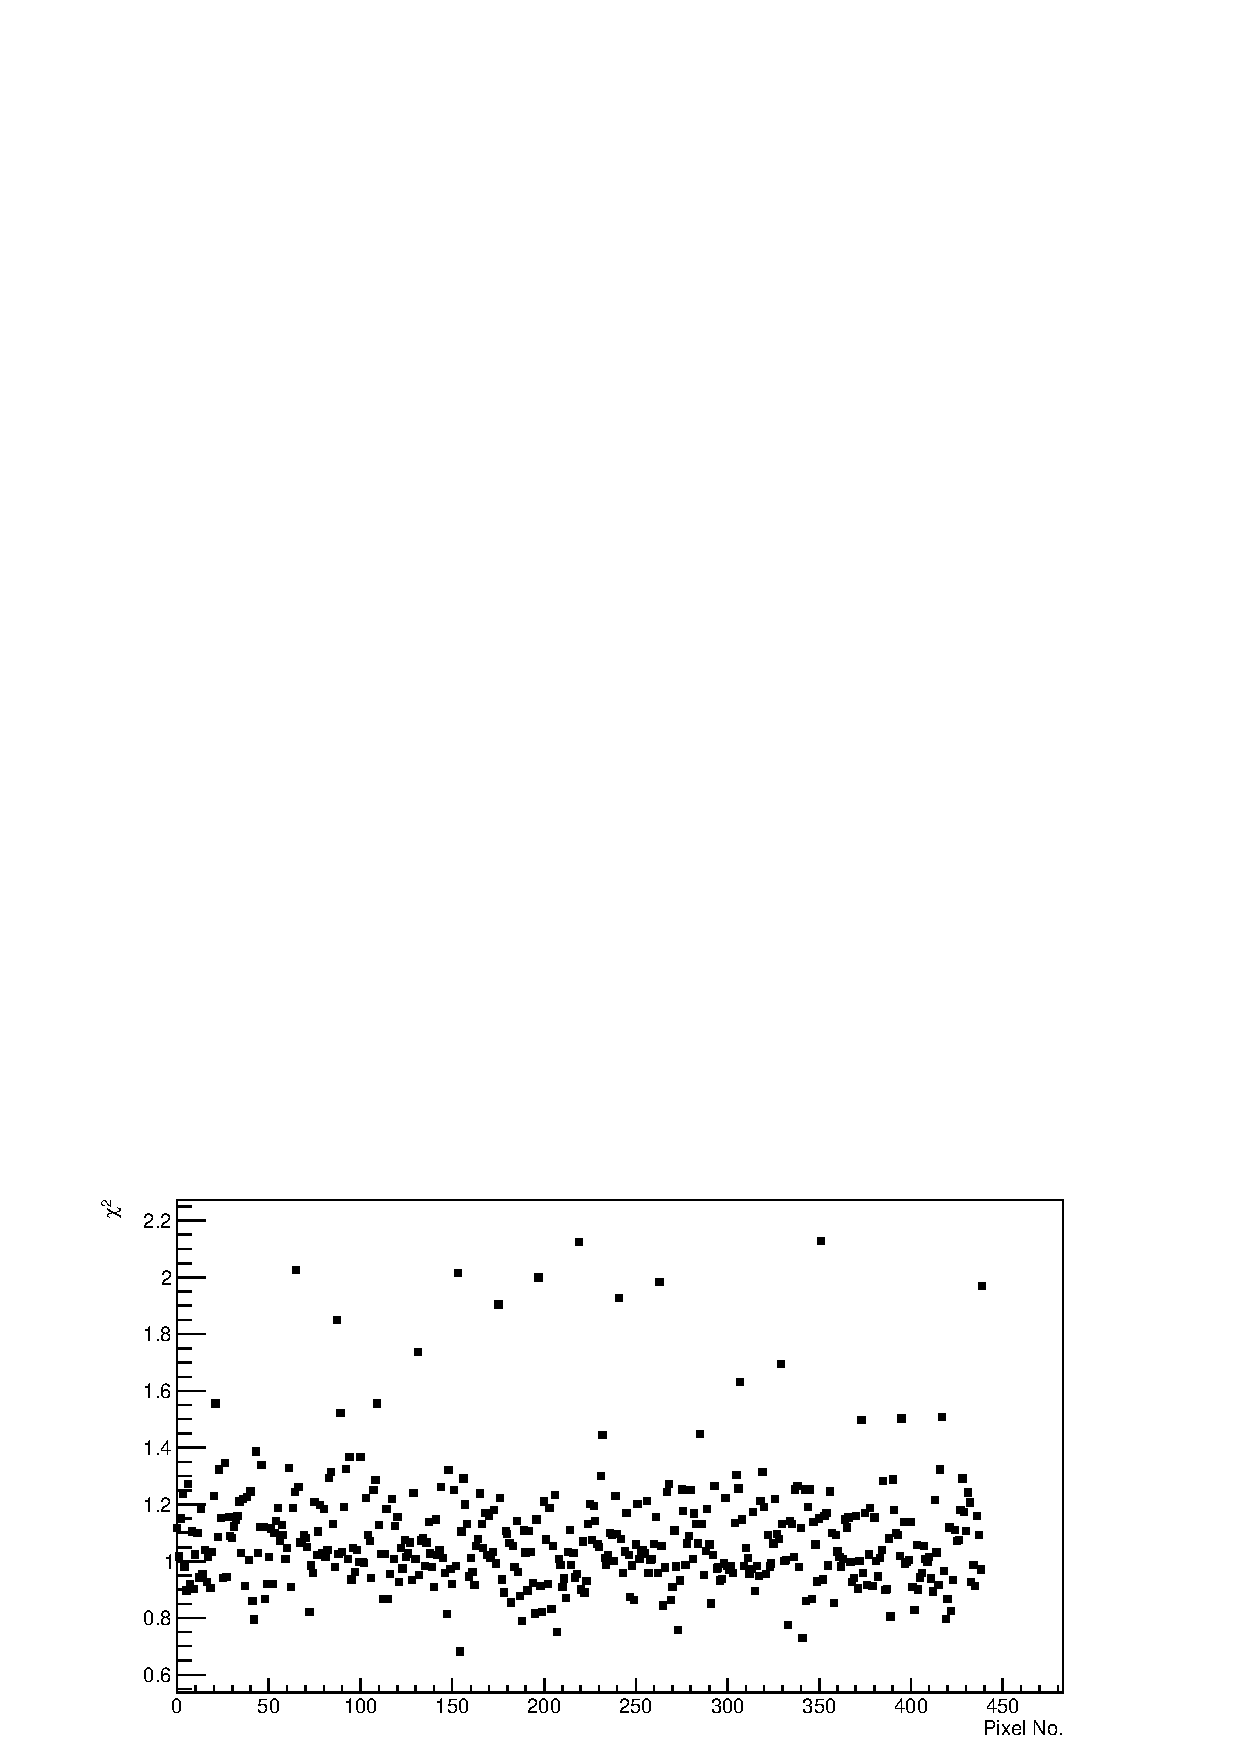
\includegraphics[width=\textwidth]{chapters/graphs/GainVarsMeas/LL_m04_2016-06-11/Set0and2/Chi2_AverageMethod_Noise_StandHV.pdf}
\caption{}
\vspace{3mm}
\includegraphics[width=\textwidth]{chapters/graphs/GainVarsMeas/LL_m04_2016-06-11/Set0and2/Chi2_AverageMethod_Noise_LowHV.pdf}
\caption{}
\end{figure}


\begin{figure} % Gain Variance Plot
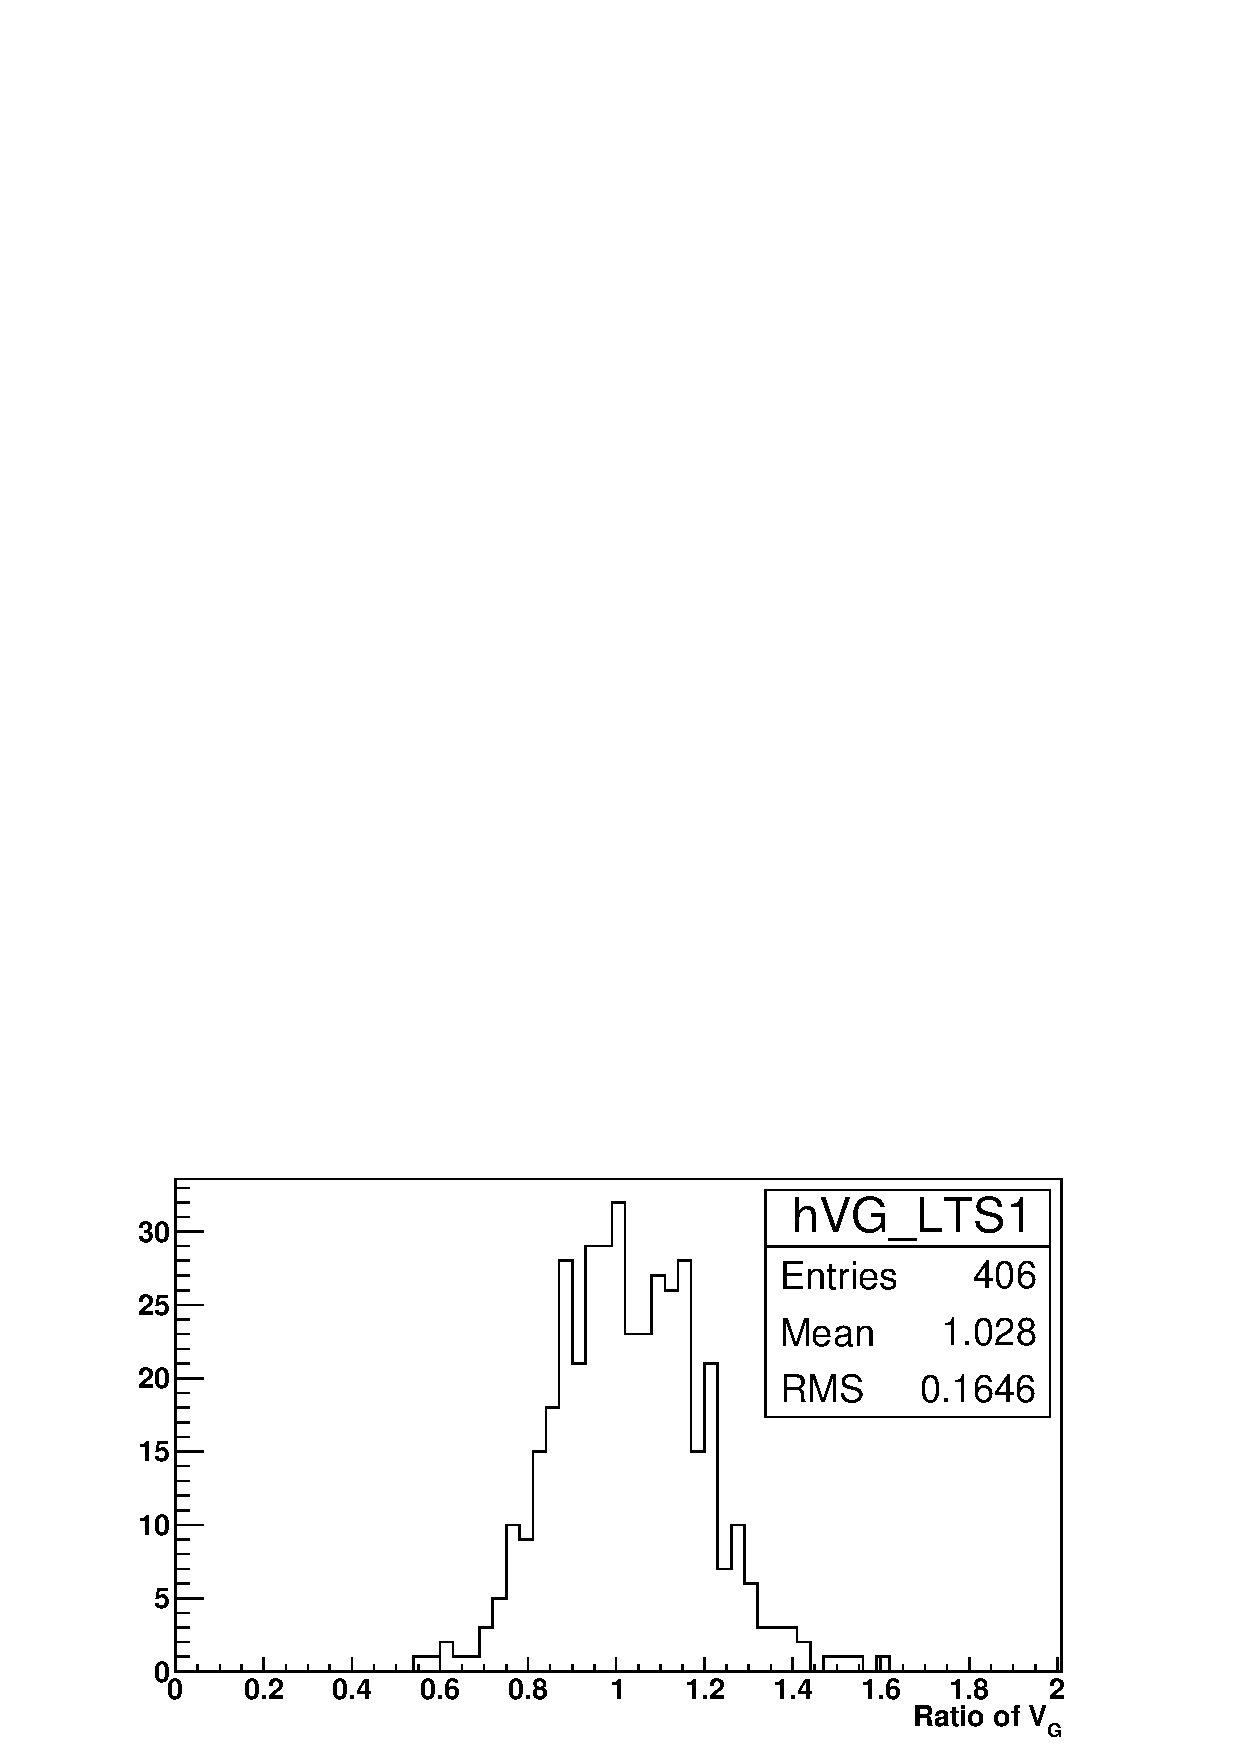
\includegraphics[width=\textwidth]{chapters/graphs/GainVarsMeas/LL_m04_2016-06-11/Set0and2/GainVairanceHist_Average_LTS.pdf}
\caption{}
\vspace{3mm}
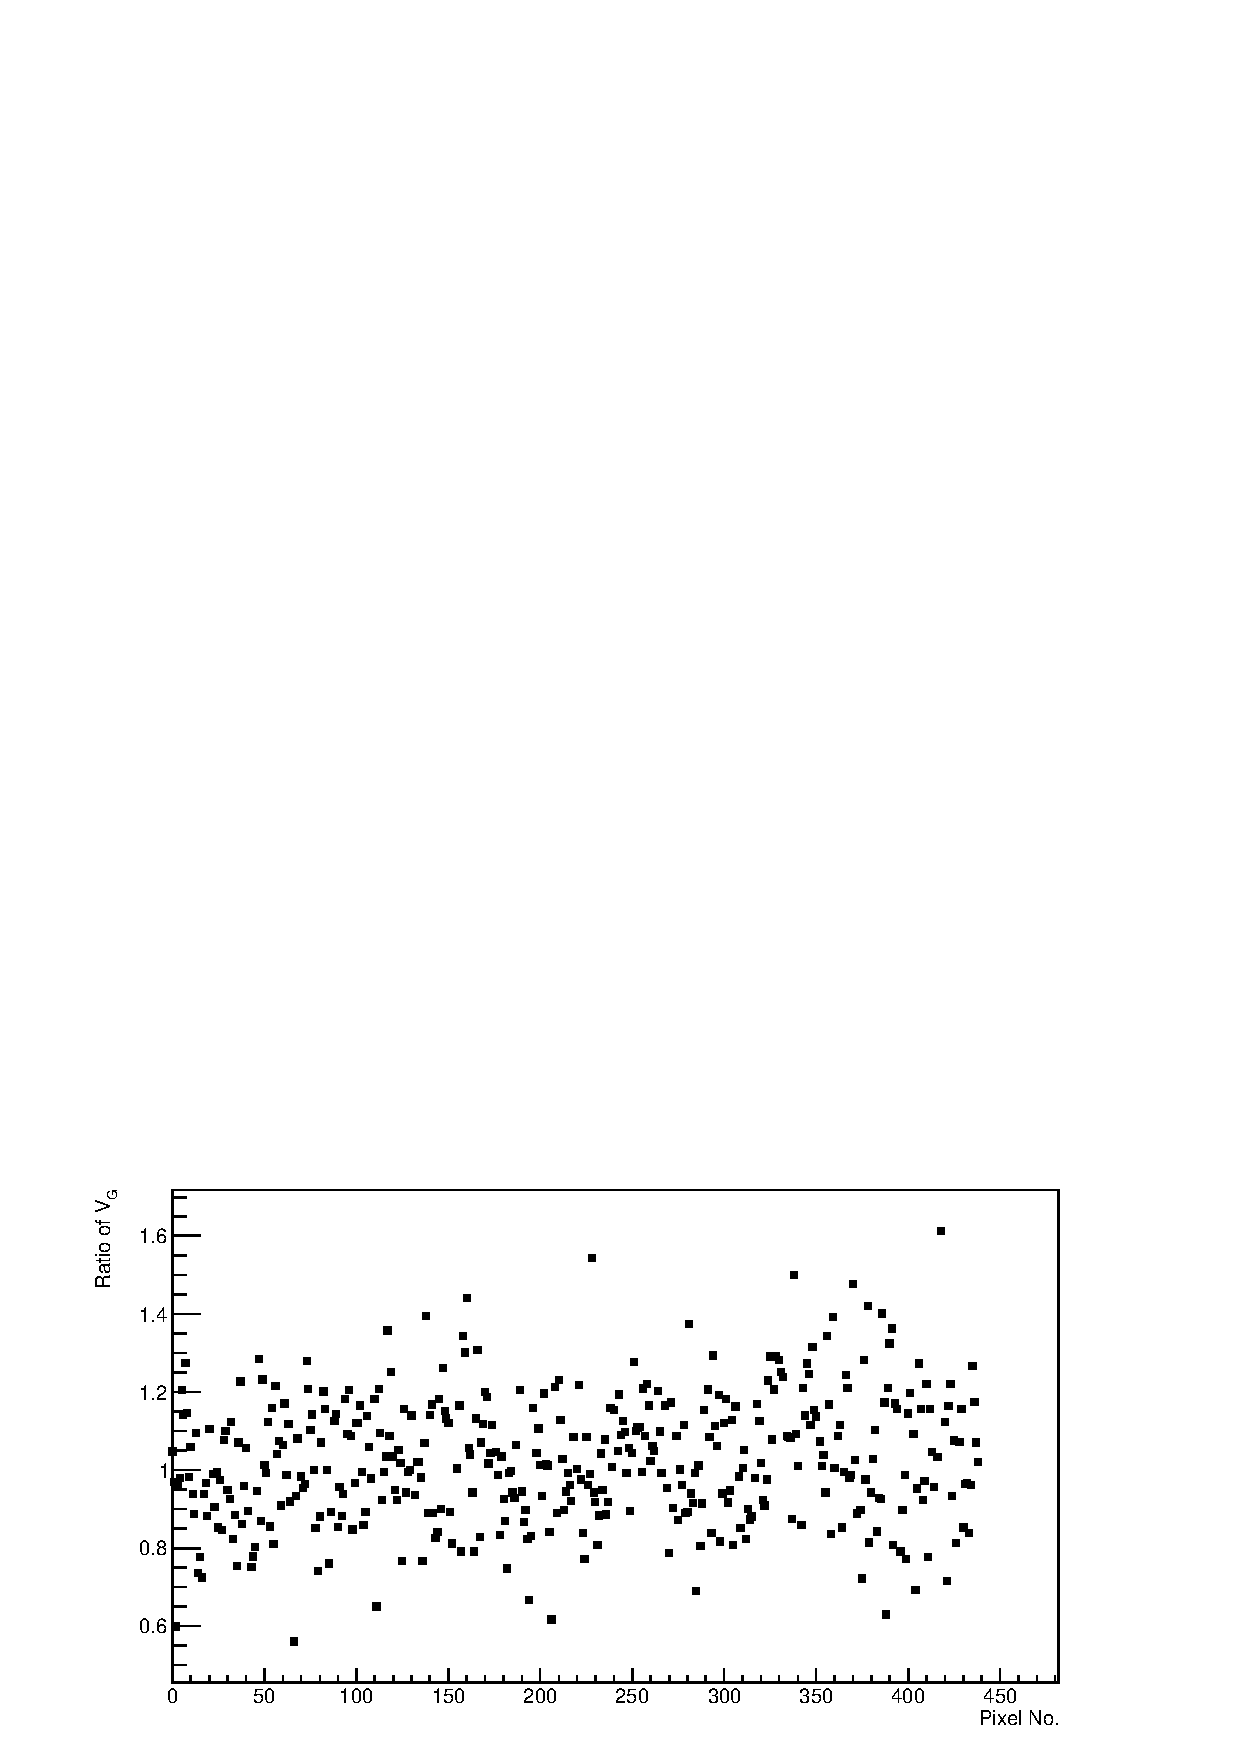
\includegraphics[width=\textwidth]{chapters/graphs/GainVarsMeas/LL_m04_2016-06-11/Set0and2/GainVars_Vs_Pixel_GainVariance_AverageLTS_Set0and2.pdf}
\caption{}
\end{figure}

\section{Result of Averaging Sets of Traces Method using Noise Distribution}

\begin{figure} % Gain Variance Plot
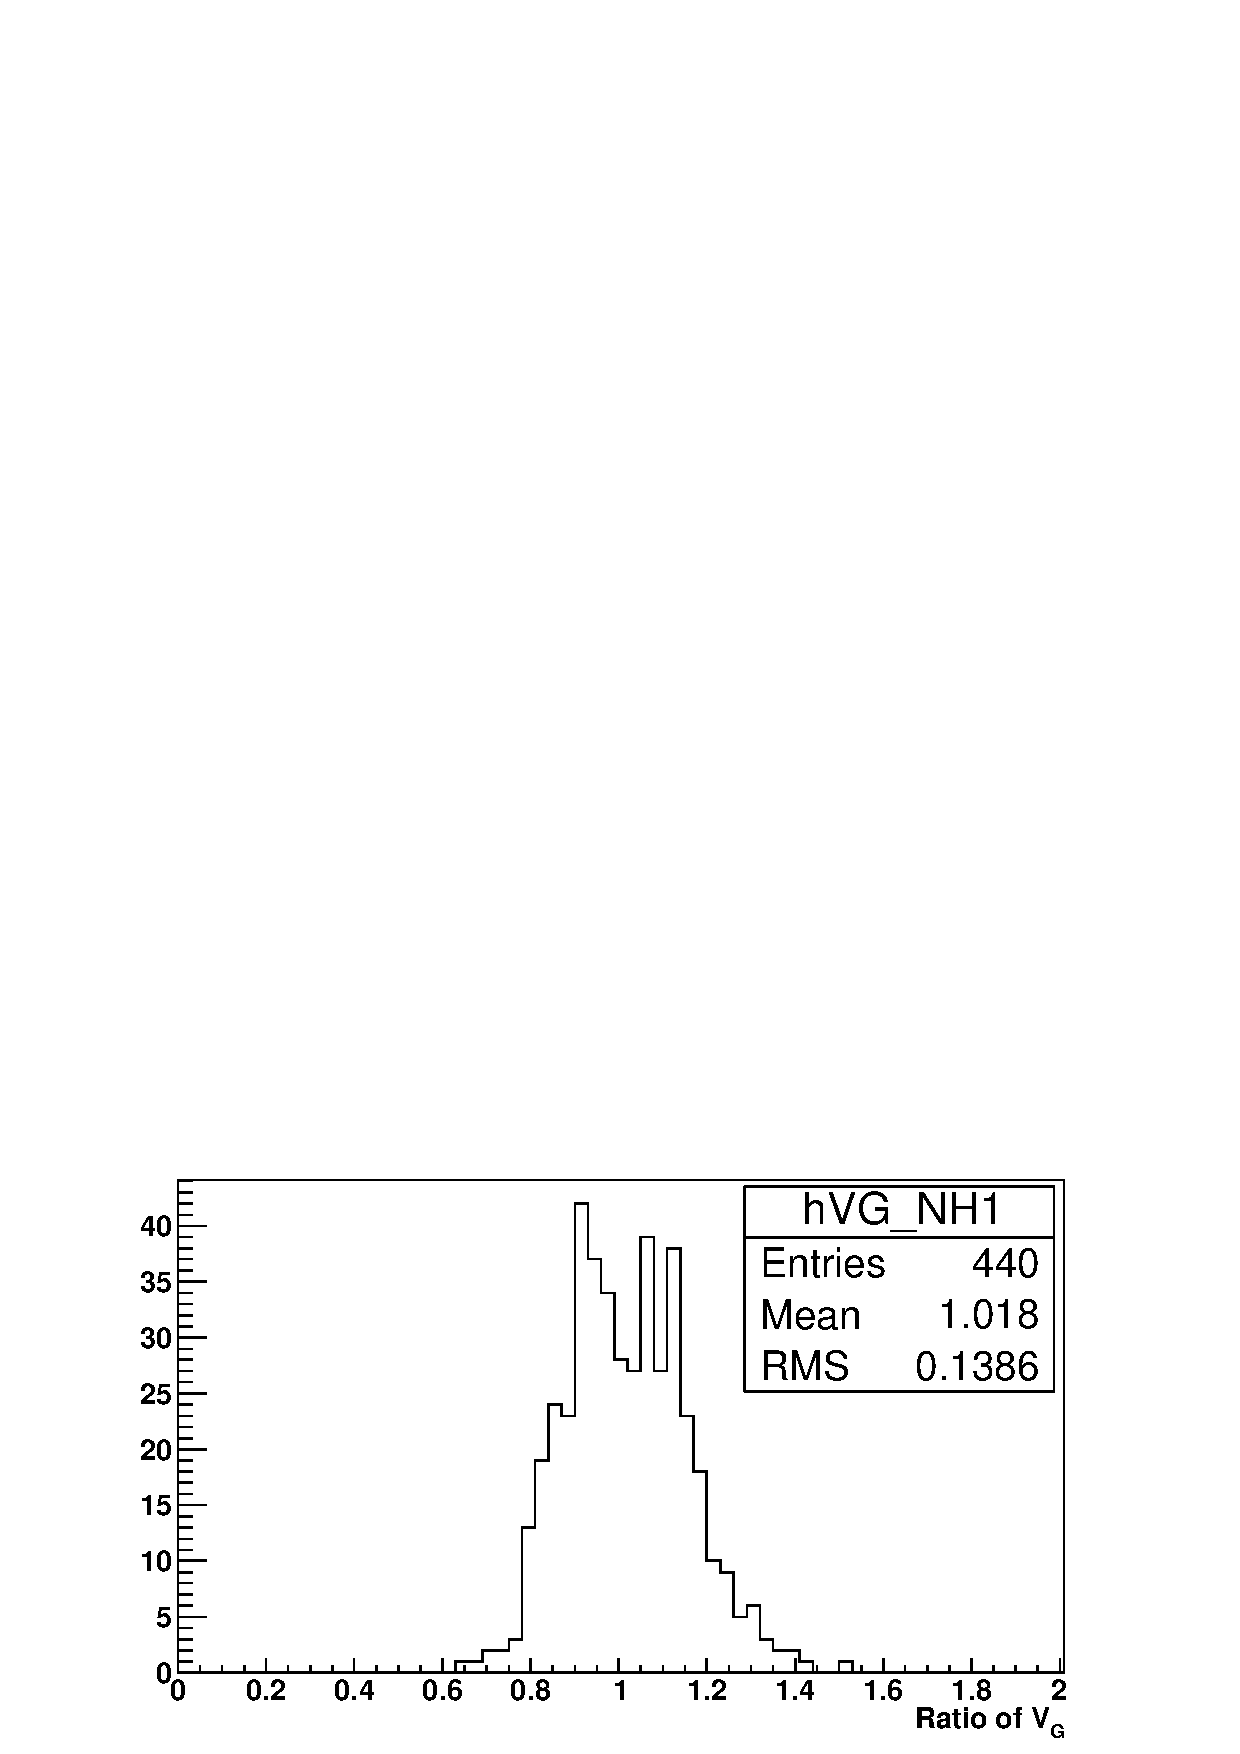
\includegraphics[width=\textwidth]{chapters/graphs/GainVarsMeas/LL_m04_2016-06-11/Set0and2/GainVairanceHist_Average_Method2.pdf}
\caption{}
\vspace{3mm}
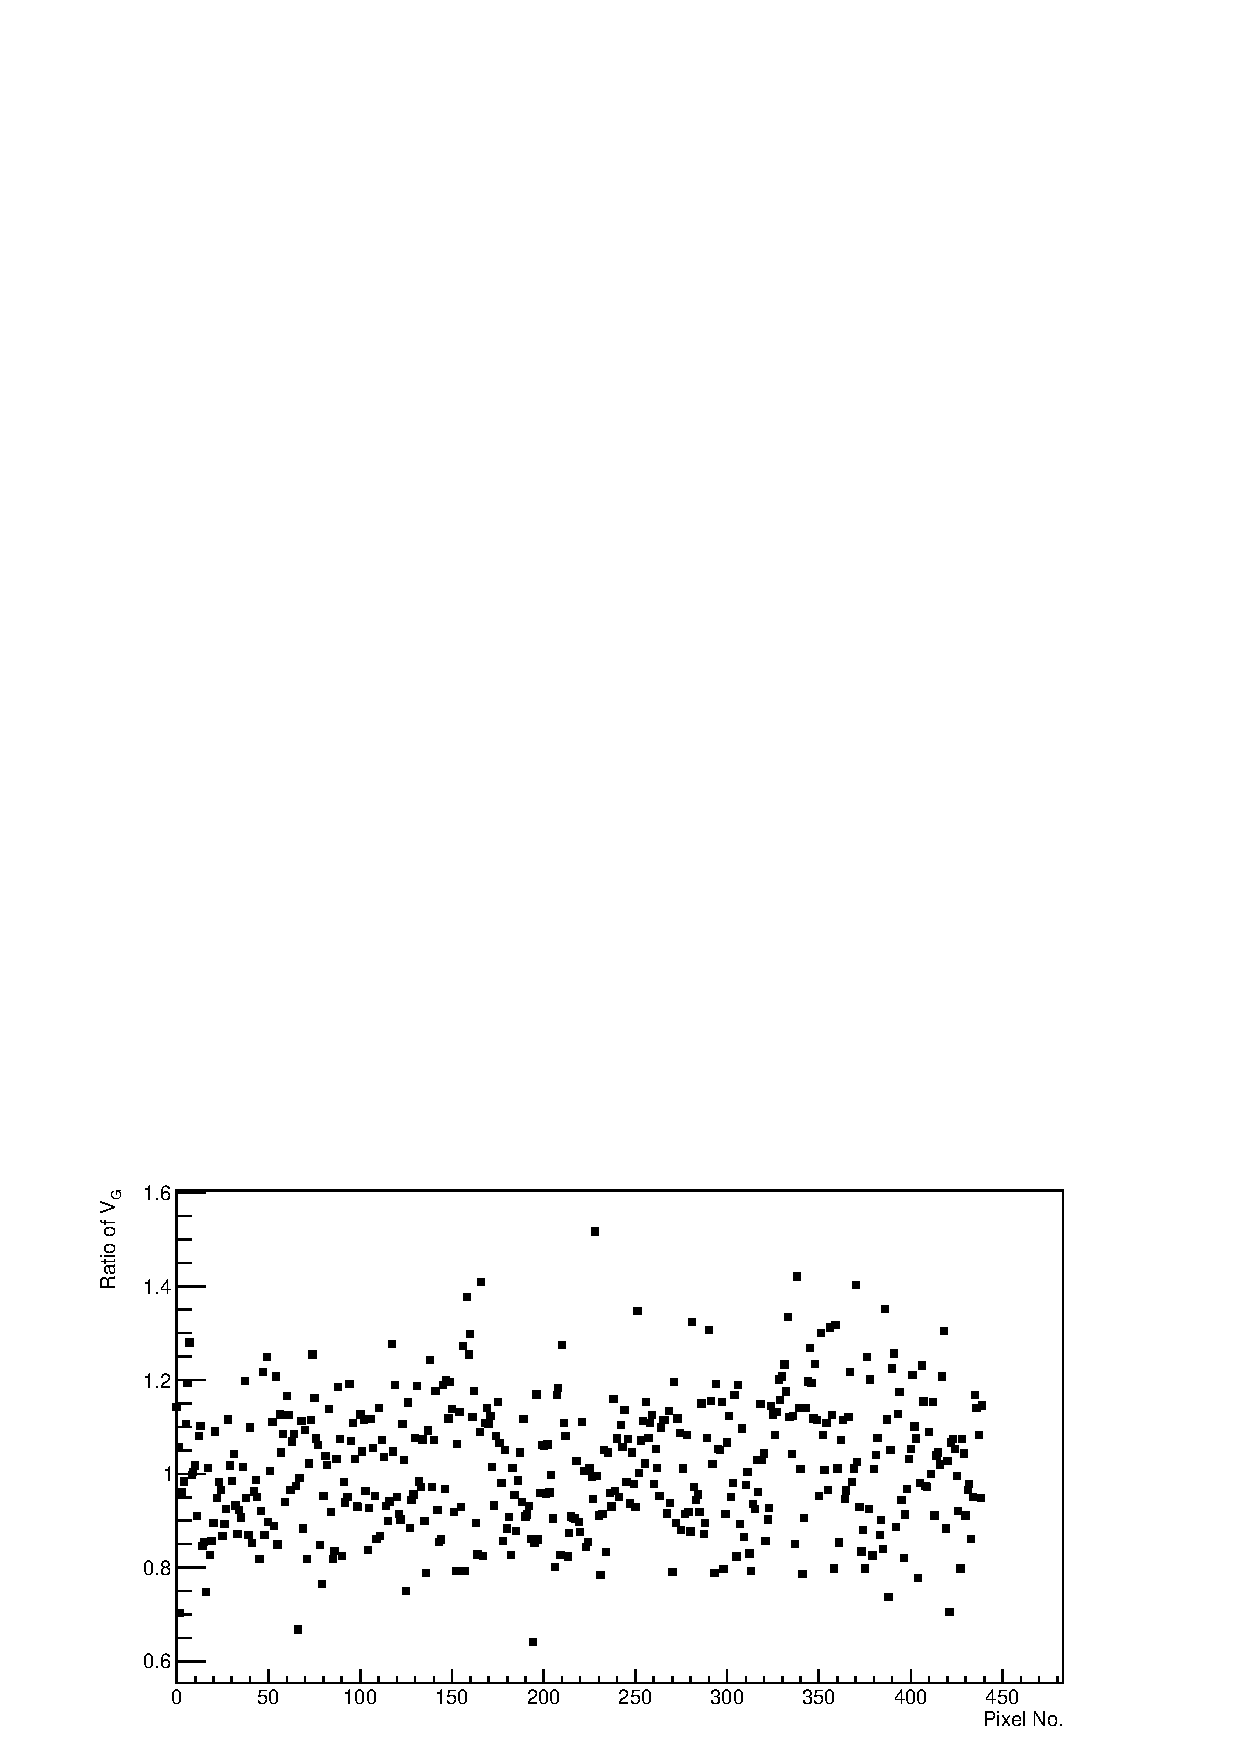
\includegraphics[width=\textwidth]{chapters/graphs/GainVarsMeas/LL_m04_2016-06-11/Set0and2/GainVars_Vs_Pixel_GainVariance_Average_Method2_Set0and2.pdf}
\caption{}
\end{figure}

\section{Attempts to measure Gain Variance in Lab at University of Adelaide}